\documentclass{article}
\usepackage{assumptionsofphysics}
\usepackage{graphicx}
\graphicspath{{images/}}
\usepackage{tikz}
\usetikzlibrary{shapes,backgrounds}
\usepackage{pgfplots}



\title{From Two Assumptions to Hamilton's Mechanics}
\author{Ryan Cosper\\
	\and
	Gabriele Carcassi}
	
\begin{document}

\maketitle

\section{Introduction}

	The purpose of this work is to re-derive Hamiltonian and Lagrangian mechanics. Historically the basis for the laws of physics were generalized experiences. These laws were rooted in the physical world rather than a mathematical one. As they are treated now, Hamiltonian and Lagrangian mechanics lack this physicality. They are taught as mathematical reformulations of Newtonian Mechanics which they are not. Many popular mechanics textbooks contain passages like this from Thorton and Marion's \textit{Classical Mechanics of Particles and Systems}: "... we need not formulate a \textit{new} theory of mechanics--the Newtonian theory is quite correct--but only devise an alternate method of dealing with complicated problems\cite{thornton_marion_2014}." This assumption of an equivalence between Newtonian and Hamiltonian mechanics is a misconception. In fact, the relationship between our three favorite classical theories is best described by figure one.
	
	 This work will begin with basic physical assumptions about a system in order to show it obeys Hamiltonian Mechanics with a more physical justification. We will start with physical assumptions, then translate those assumptions into precise mathematical definitions. This will lead us to our results. 	
	 
\begin{figure}[!!ht]
\begin{center}
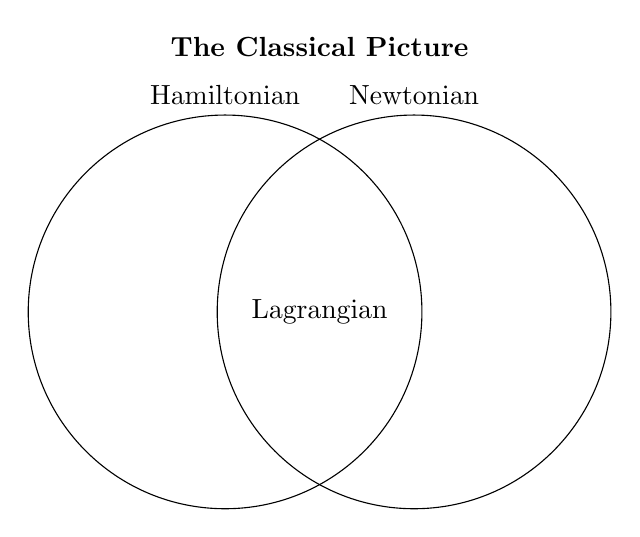
\begin{tikzpicture}

\node [label={\textbf{The Classical Picture}}] (C) at (1.2,3){};
 
% Set A
\node [draw,
    circle,
    minimum size =5cm,
    label={90:Hamiltonian}] (A) at (0,0){};
 
% Set B
\node [draw,
    circle,
    minimum size =5cm,
    label={90:Newtonian}] (B) at (2.4,0){};
 
% Set intersection label
\node at (1.2,0) {Lagrangian};
 
\end{tikzpicture}
\end{center}
\caption{Venn diagram showing the relationship between our three favorite classical theories.}
\end{figure}

\section{Infinitesimal Reducibility}
	
\begin{assump}[Infinitesimal reducibility]
	The state of the system is reducible to the state of its infinitesimal parts. That is, giving the state of the whole system is equivalent to giving the state of its parts, which in turn is equivalent to giving the state of its subparts and so on. This relationship holds the the other way as well. Giving the states of the smallest subdivisions of the system is equivalent to giving the state of the whole system.
\end{assump}
	
	%\emph{Explain in practical terms what reducibility is}
	
	What does it mean physically for a system to be reducible? This first assumption that underlies classical mechanics prescribes how a system can be broken down into its component parts. This assumption will provide us with a mathematical framework to describe the state of the system we are investigating.
	
	Let's consider a ball that we throw through the air. This ball will follow some path. We assume we can fully describe the state of the ball by its motion through the air. Now, suppose we draw a red dot on this ball. Then if we fully describe the motion of the ball, we have also equivalently described the motion of the red dot. The ball is a reducible system meaning knowledge of the state of the whole is equivalent to knowledge of the states of the parts. The internal dynamics of the system are accessible meaning we can know the states of the parts of the system given knowledge of the state of the whole. Additionally if we give the motion of all possible red dots on the surface of the ball, we know the motion of the whole ball. The state of the whole system can be known from the states of its parts. 
	
\begin{figure}[!ht]
\centerline{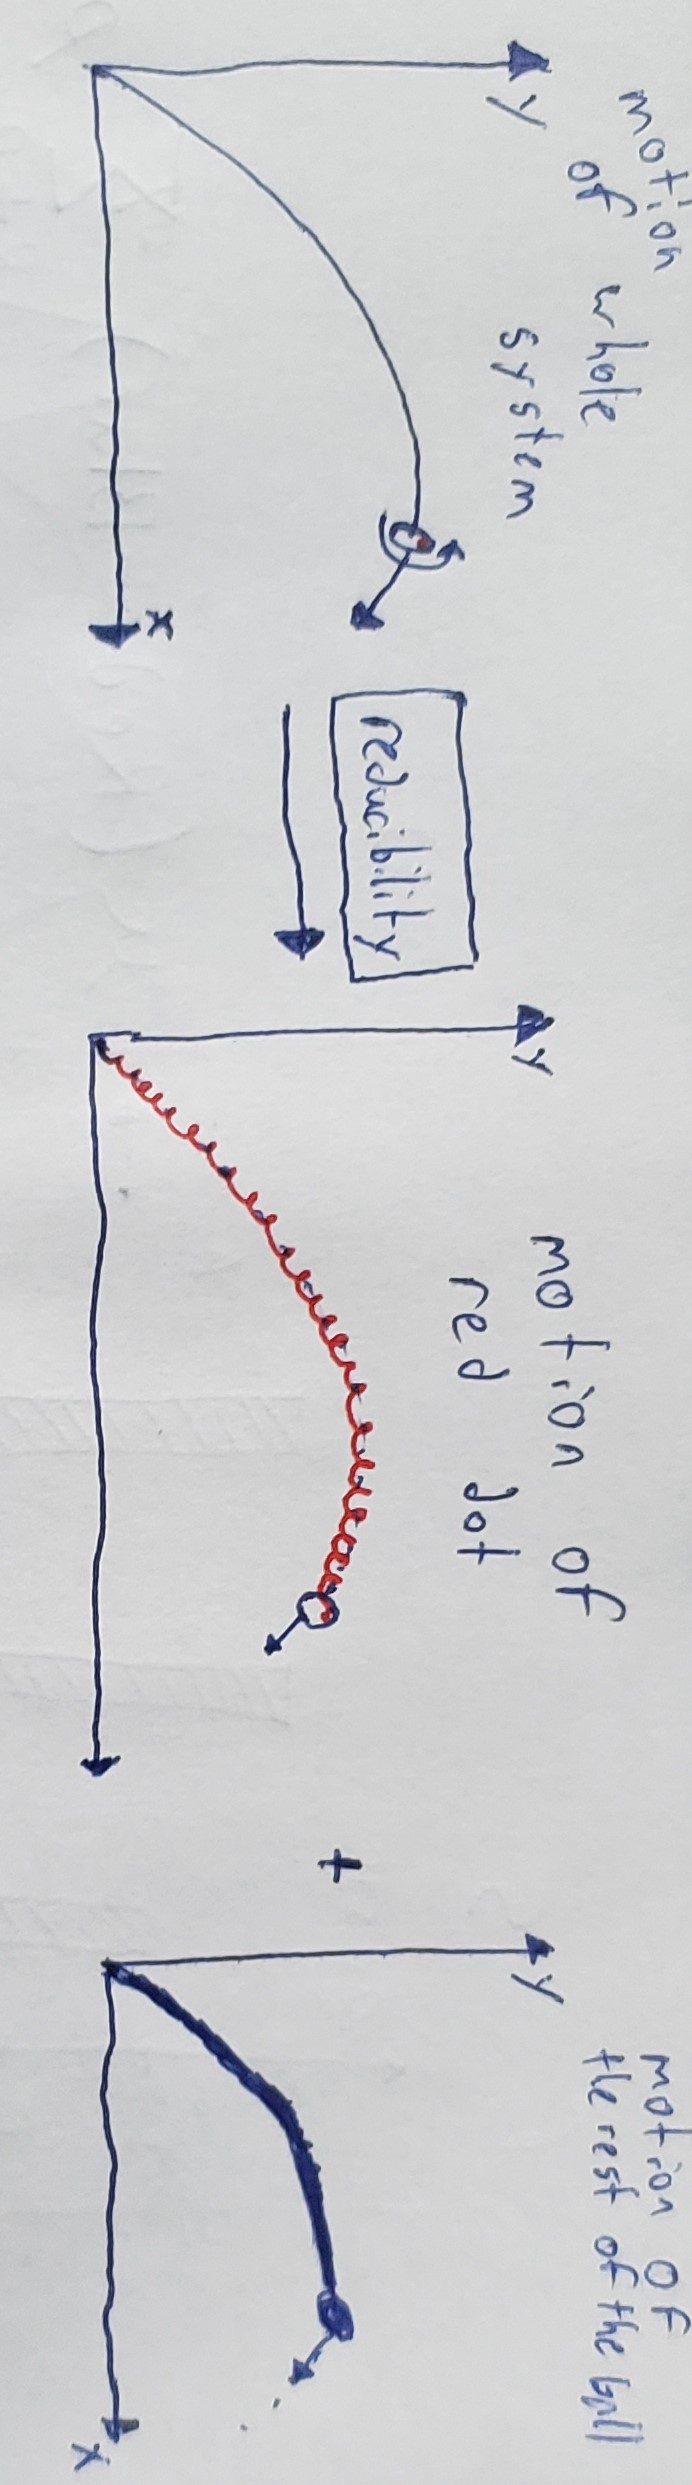
\includegraphics[width=\linewidth,angle=90,scale=.25]{reddotdiagram.jpg}}
\caption{Motion of our ball and red dot example. Because this system is reducible we can break the whole system into its parts.}
\end{figure}

	%\emph{motivate the uniqueness of the distribution}	
	
	Each state of the whole system is uniquely determined by the states of its parts, meaning that given the state of all parts, we can determine exactly the state of the whole system. Two identical systems are in the same state if and only if all of their parts are in the same states. The same is true the other way around. The states of the parts of the system are uniquely determined by the state of the whole. Thus we have an invertible map between the state of our whole system and the states of its parts. In our example, this means that there is exactly one path traveled by the red dot per distinct state of the whole ball. So if we throw the ball with no angular velocity, the red dot will travel a parabola through the air. We could then throw the ball with the same linear velocity so that its center of mass travels the same path as before, but if the ball is spinning we have a different path traveled by the red dot. So from two distinct states of the overall system, one with angular velocity one without, we find two distinct sets of states of the parts of the system. One spiraling trajectory and one parabola.
		
	 %If we consider a ball of irreducible material i.e. an electron, we cannot describe the state of a dot drawn on its surface. We could not say for instance that a photon scattering with that electron interacts specifically with the part of the electron with the dot. That is because the electron is not reducible; we cannot describe the state of the electron by breaking it into smaller parts and describing those parts. We cannot describe a process in which something interacts with only part of the electron. 
	 
	 %\emph{Describe what the process of subdivision is, and define the particle as the limit of that process}
	 
	 We have described reducibility in general, but what does it mean to be infinitesimally reducible? If a system is infinitesimally reducible we can subdivide it as many times as we want and the smallest subdivisions will still be themselves reducible. If we imagine that we divide our system until we approach the limit of recursive subdivision we will arrive at a collection of infinitesimally small parts of the system; we call these smallest subdivisions classical particles. What does this mean physically? Continuing our previous example, imagine we cover the surface of the ball in red dots. We then remove these dots and replace each of them with a number of smaller dots. We repeat this process until the radius of the dots is approaching zero. Because the ball is a reducible system, given the state of the whole ball, we know the states of all of the red dots drawn on it. It is important to note that the dots do not ever become points. They are always have radii that are greater than zero. No dot is a point particle, rather they are infinitesimally small subdivisions. We can always divide them again.
	 
	 The limit of these subdivisions are our classical particles. Assuming a system to be infinitesimally reducible means that given the state of the whole system, we can describe the states of all the infinitesimally small parts of the system. Now we must codify this idea formally.
	 	
	Let's start with a discrete system as it is conceptually simpler Consider a box with a fixed number of balls of varying colors as our whole system.\footnote{this is not an example of an infinitesimally reducible system as the balls are the limit of its reducibility, but it serves as an illustrative example.} Suppose the state of the whole system will be defined by the number of balls of each color. We can formally define the \textit{state space} of the balls as $\mathcal{S}$ which spans all possible colors. Each ball is at a point $s \in \mathcal{S}$ corresponding to its color. We call the state space of our whole system $\mathcal{C}$ which spans all possible color combinations of the balls. One state of the whole system is a point $c \in \mathcal{C}$. For a state $c \in \mathcal{C}$ we can define the number of balls of each color as a \textit{distribution}, $\rho$, over the state space $\mathcal{S}$ of the balls. This distribution is unique to each state of the whole system. Two identical systems are in the same state if and only if their distributions are equivalent. For each distinct state $c \in \mathcal{C}$ of the whole system, we have exactly one $\rho$. 

\begin{figure}[!ht]
\centerline{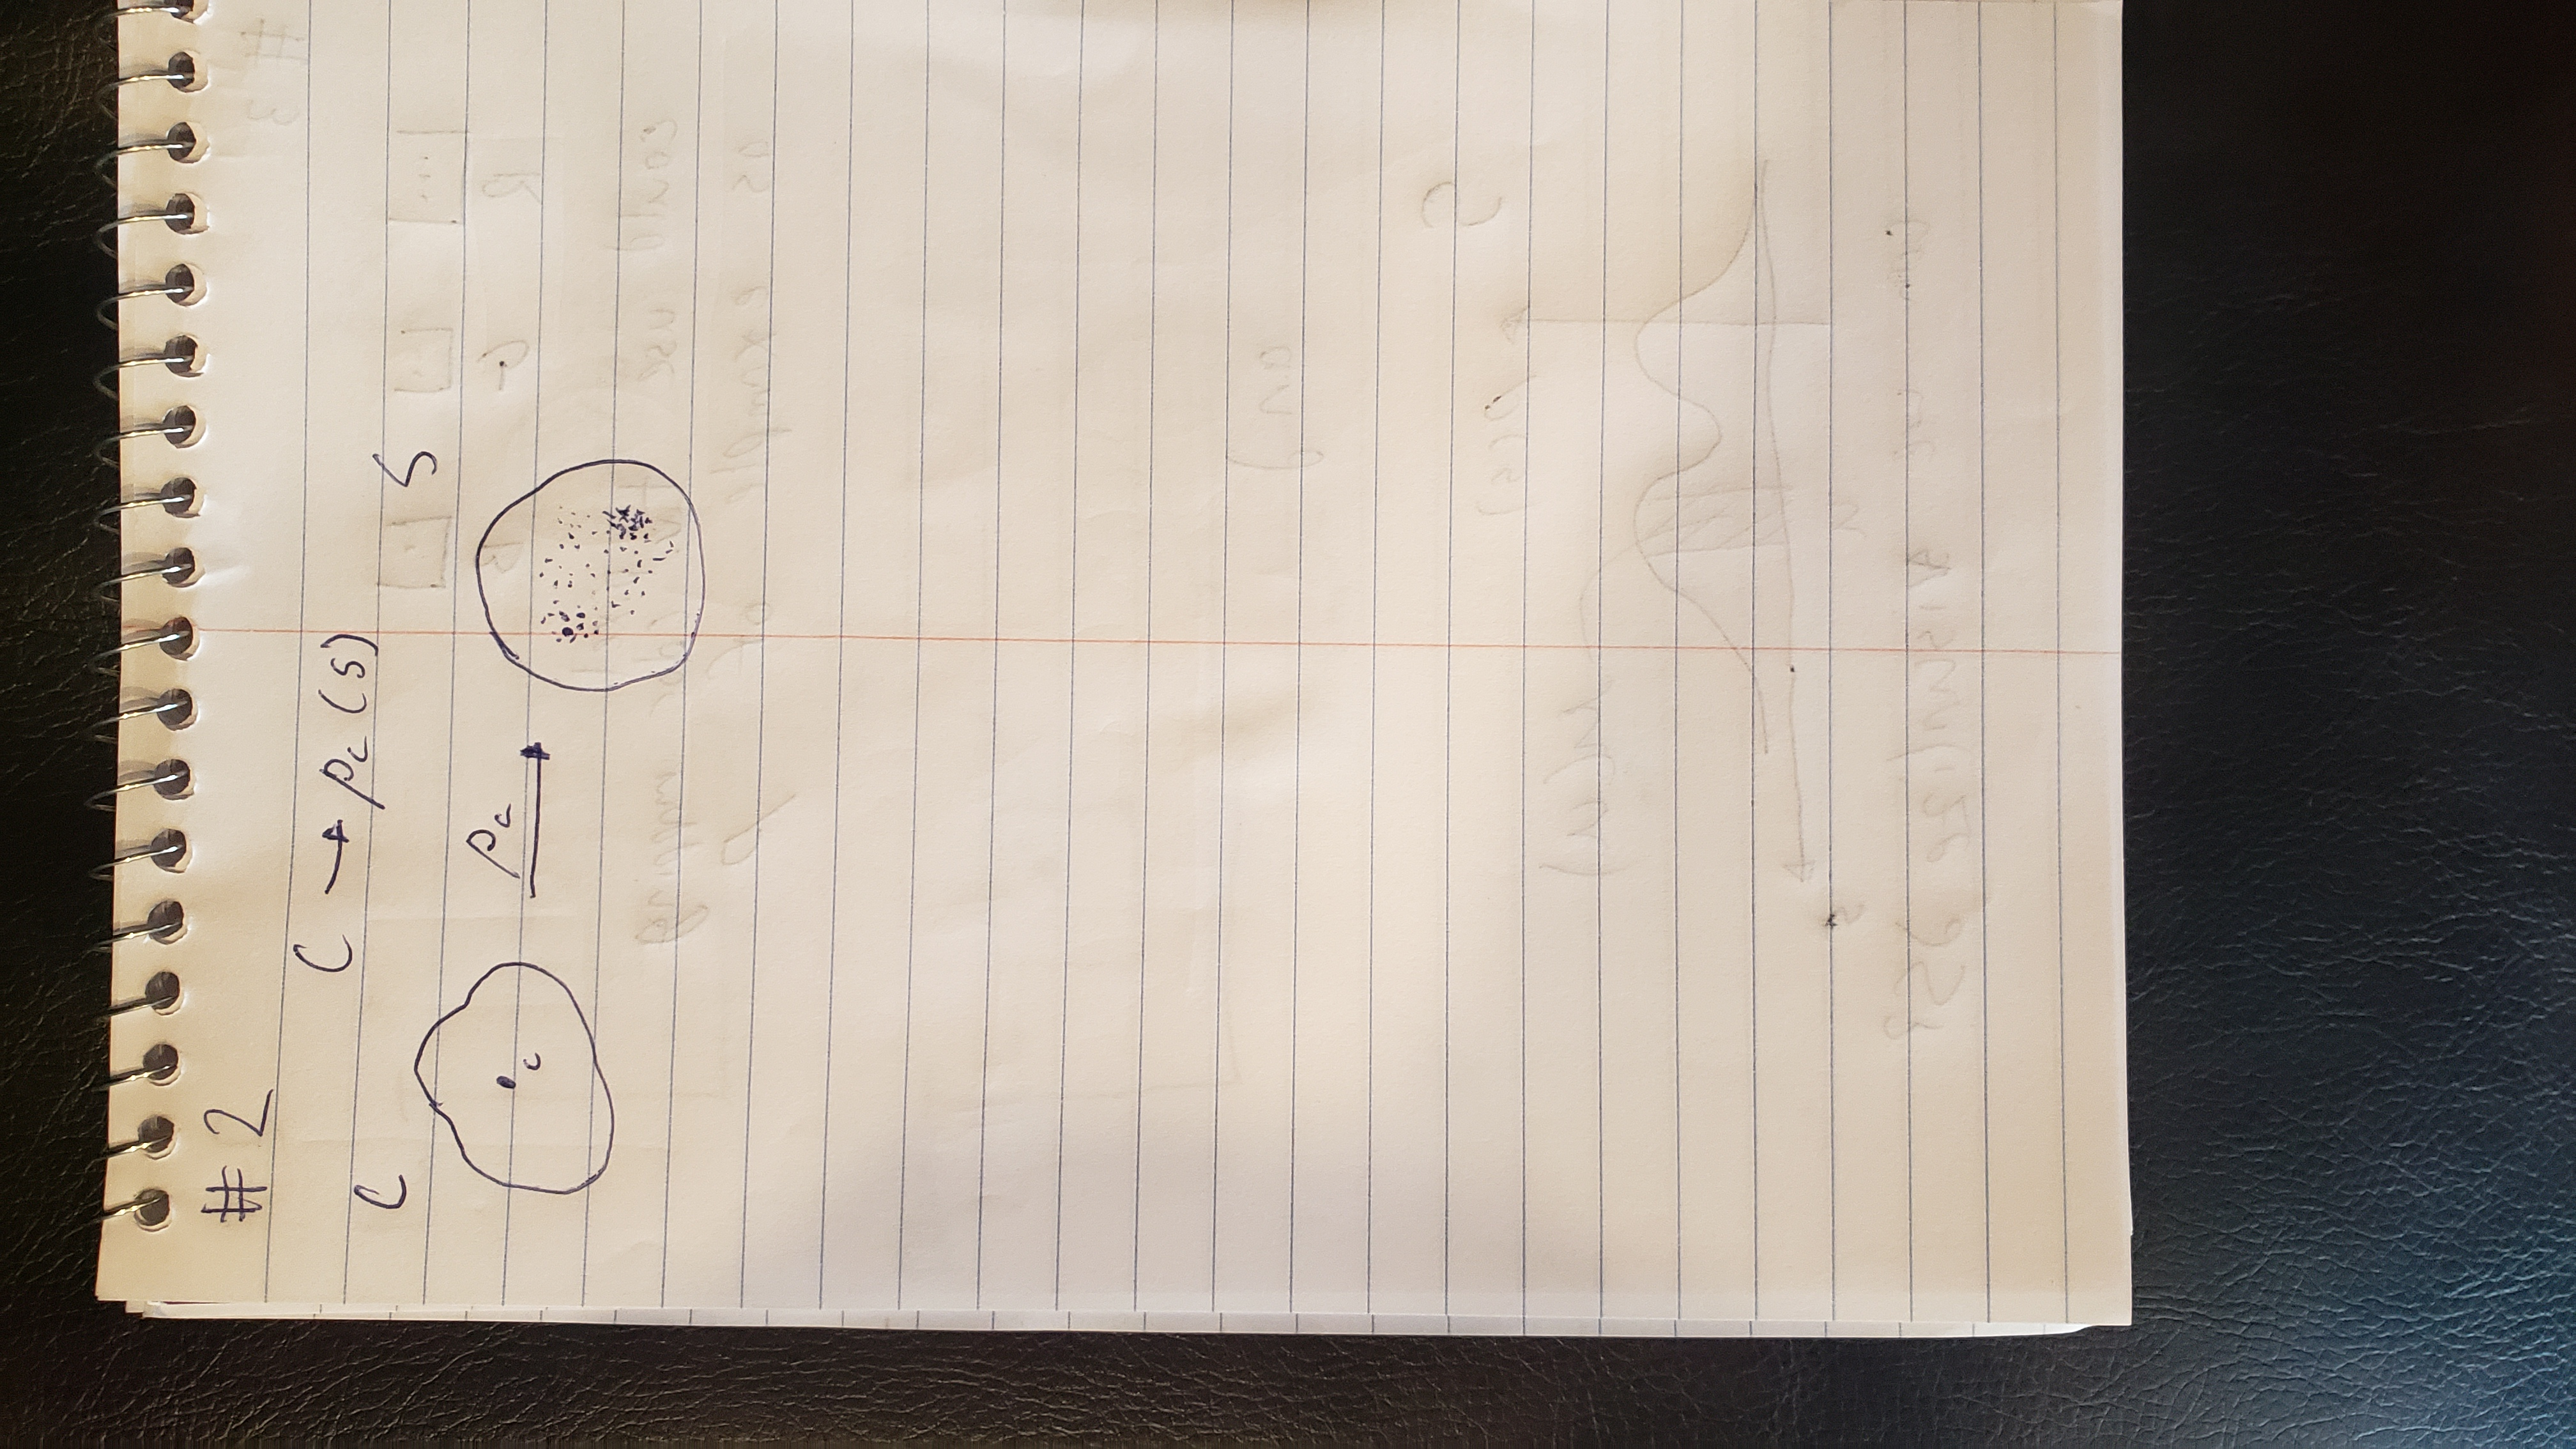
\includegraphics[width=\textwidth,angle=-90,scale=.35]{diagram2.jpg}}
\caption{Two different states of the system map to two different distributions of the parts of the system over $\mathcal{S}$.}
\end{figure}

\begin{figure}
\begin{center}
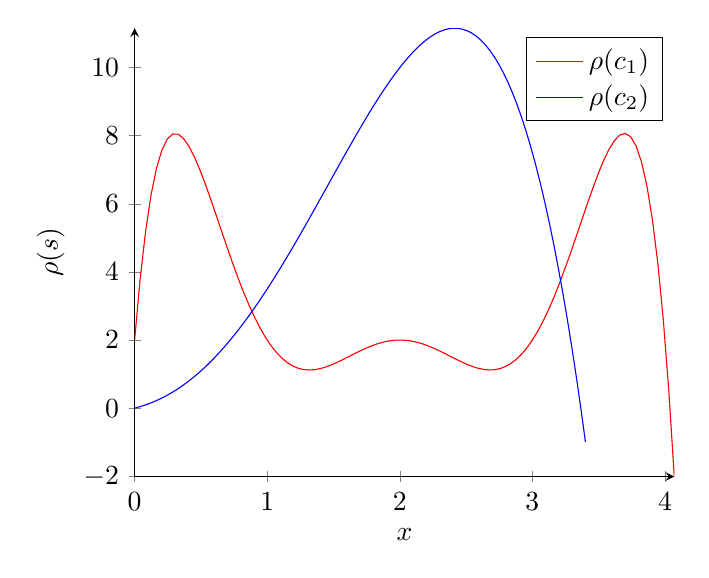
\begin{tikzpicture}
\begin{axis}[
    axis lines = left,
    xlabel = \(x\),
    ylabel = {\( \rho (s) \)},
]
%Below the red parabola is defined
\addplot [
    domain=0:4.07, 
    samples=100, 
    color=red,
]
{-1*x^6+12*x^5-55*x^4+120*x^3-124*x^2+48*x+2};
\addlegendentry{\( \rho (c_1) \)}

\addplot [
    domain=0:3.4, 
    samples=100, 
    color=blue,
]
{-.5*x^4+x+x^3+2*x^2};
\addlegendentry{\( \rho (c_2) \)}


\end{axis}
\end{tikzpicture}
\end{center}
\caption{Two different states of the system map to two different distributions of the parts of the system over $\mathcal{S}$.}
\end{figure}
	
	For each subset of colors in $\mathcal{S}$, we can count the number balls that are those colors; call this counting function $\mu : \mathcal{S} \to \mathbb{R}$. That is, for each $U \subset \mathcal{S}$ we have $\mu(U) = \sum_{s \in U} \rho(s)$. We will normalize this counting function by defining $\mu(S) = 1$.
	
\begin{figure}[!ht]
\centerline{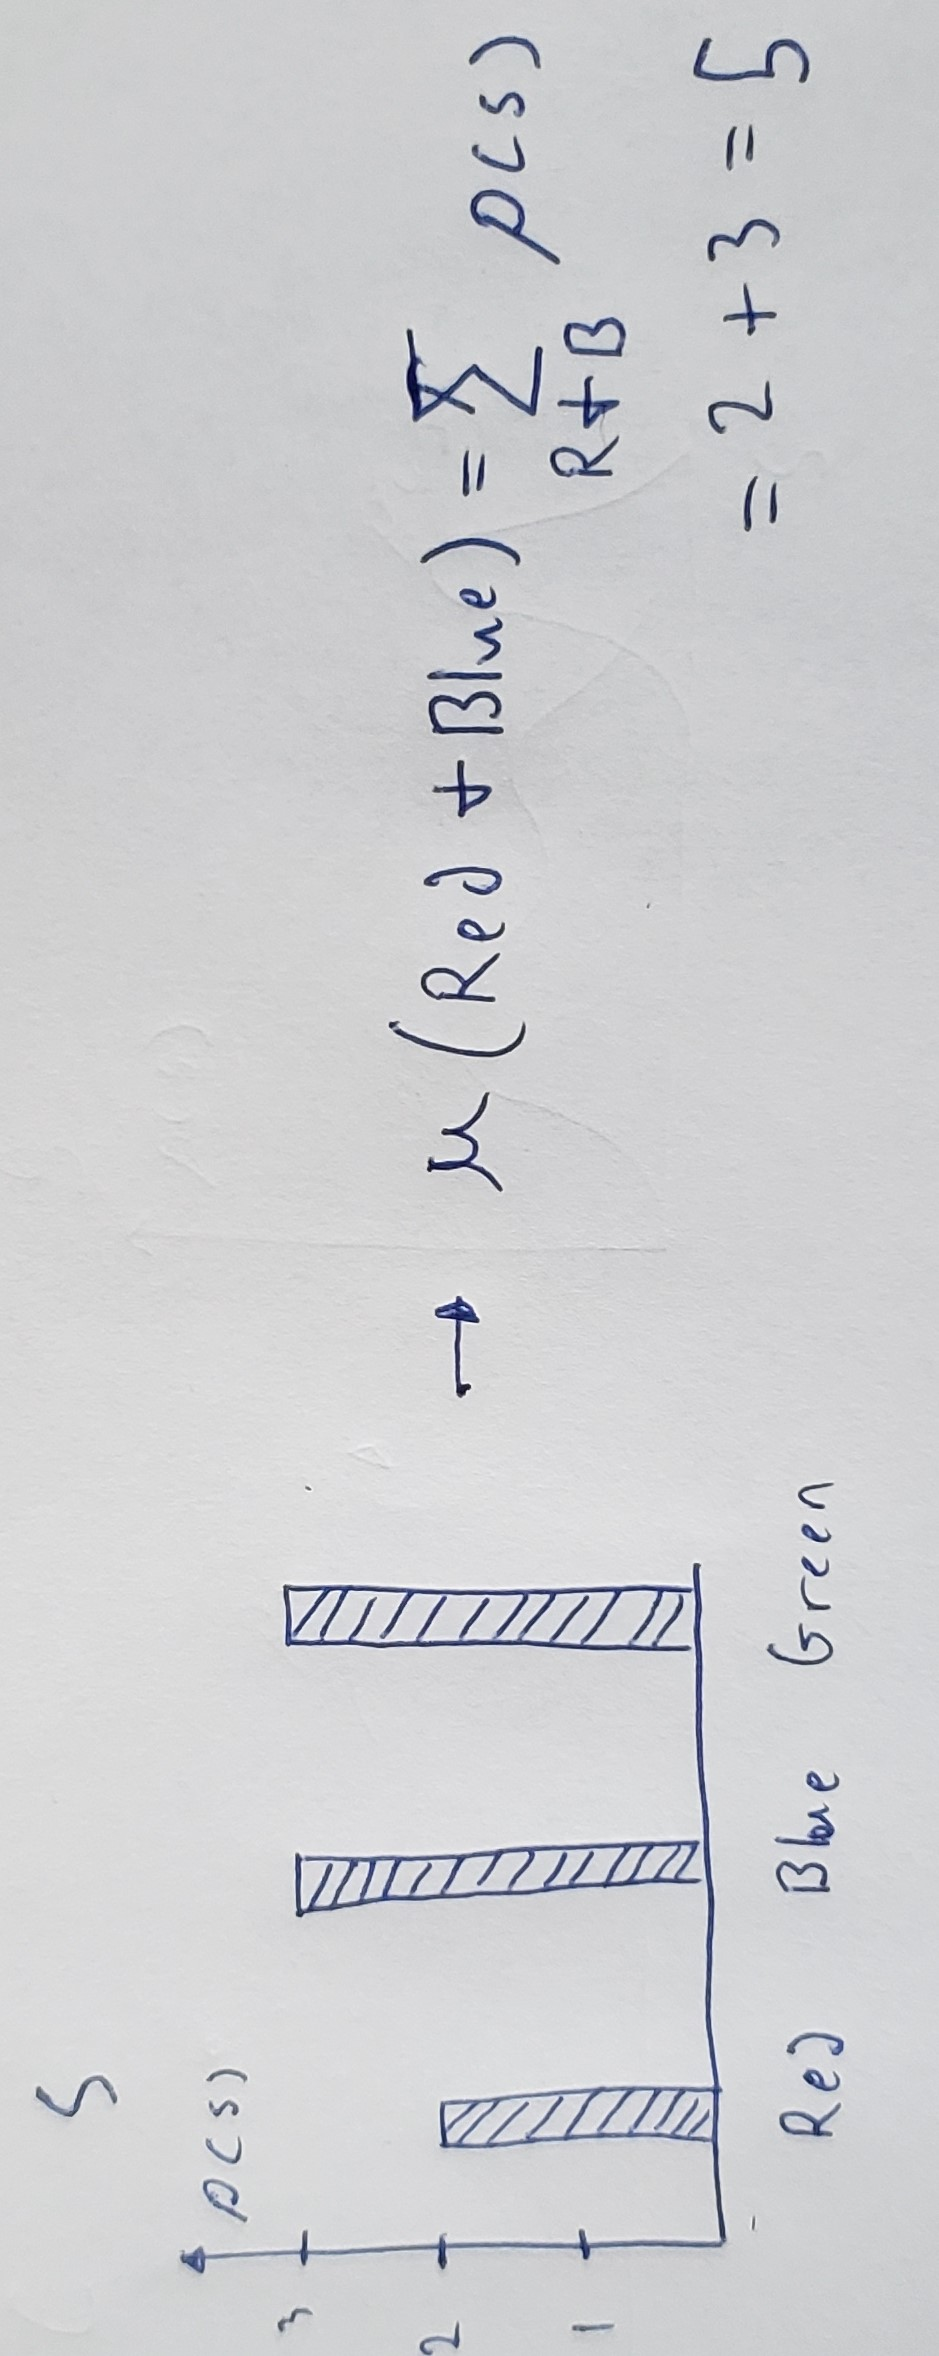
\includegraphics[width=\textwidth,angle=-90,scale=.35]{diagram3.jpg}}
\caption{Discrete example of our counting function $\mu(U)$. (not normalized)}
\end{figure}
	
	%\emph{formalize continuous case, improve example}	
	
	If our system is continuous the main ideas above hold, but we must make two changes to the formalization. First, our distribution $\rho : \mathcal{S} \to \mathbb{R}$ becomes a density of states over the space and second, for $\mu$ instead of a sum we use an integral: $\mu(U) = \int_{U} \rho(s) d\mathcal{S}$ where $d\mathcal{S}$ gives the number of states in an infinitesimal area. For a physical example let's consider a classical gas distributed in a volume. The state of the whole is the distribution. Now we can see that our counting function will count the amount of gas in a region of this volume.
\begin{figure}[!ht]
\centerline{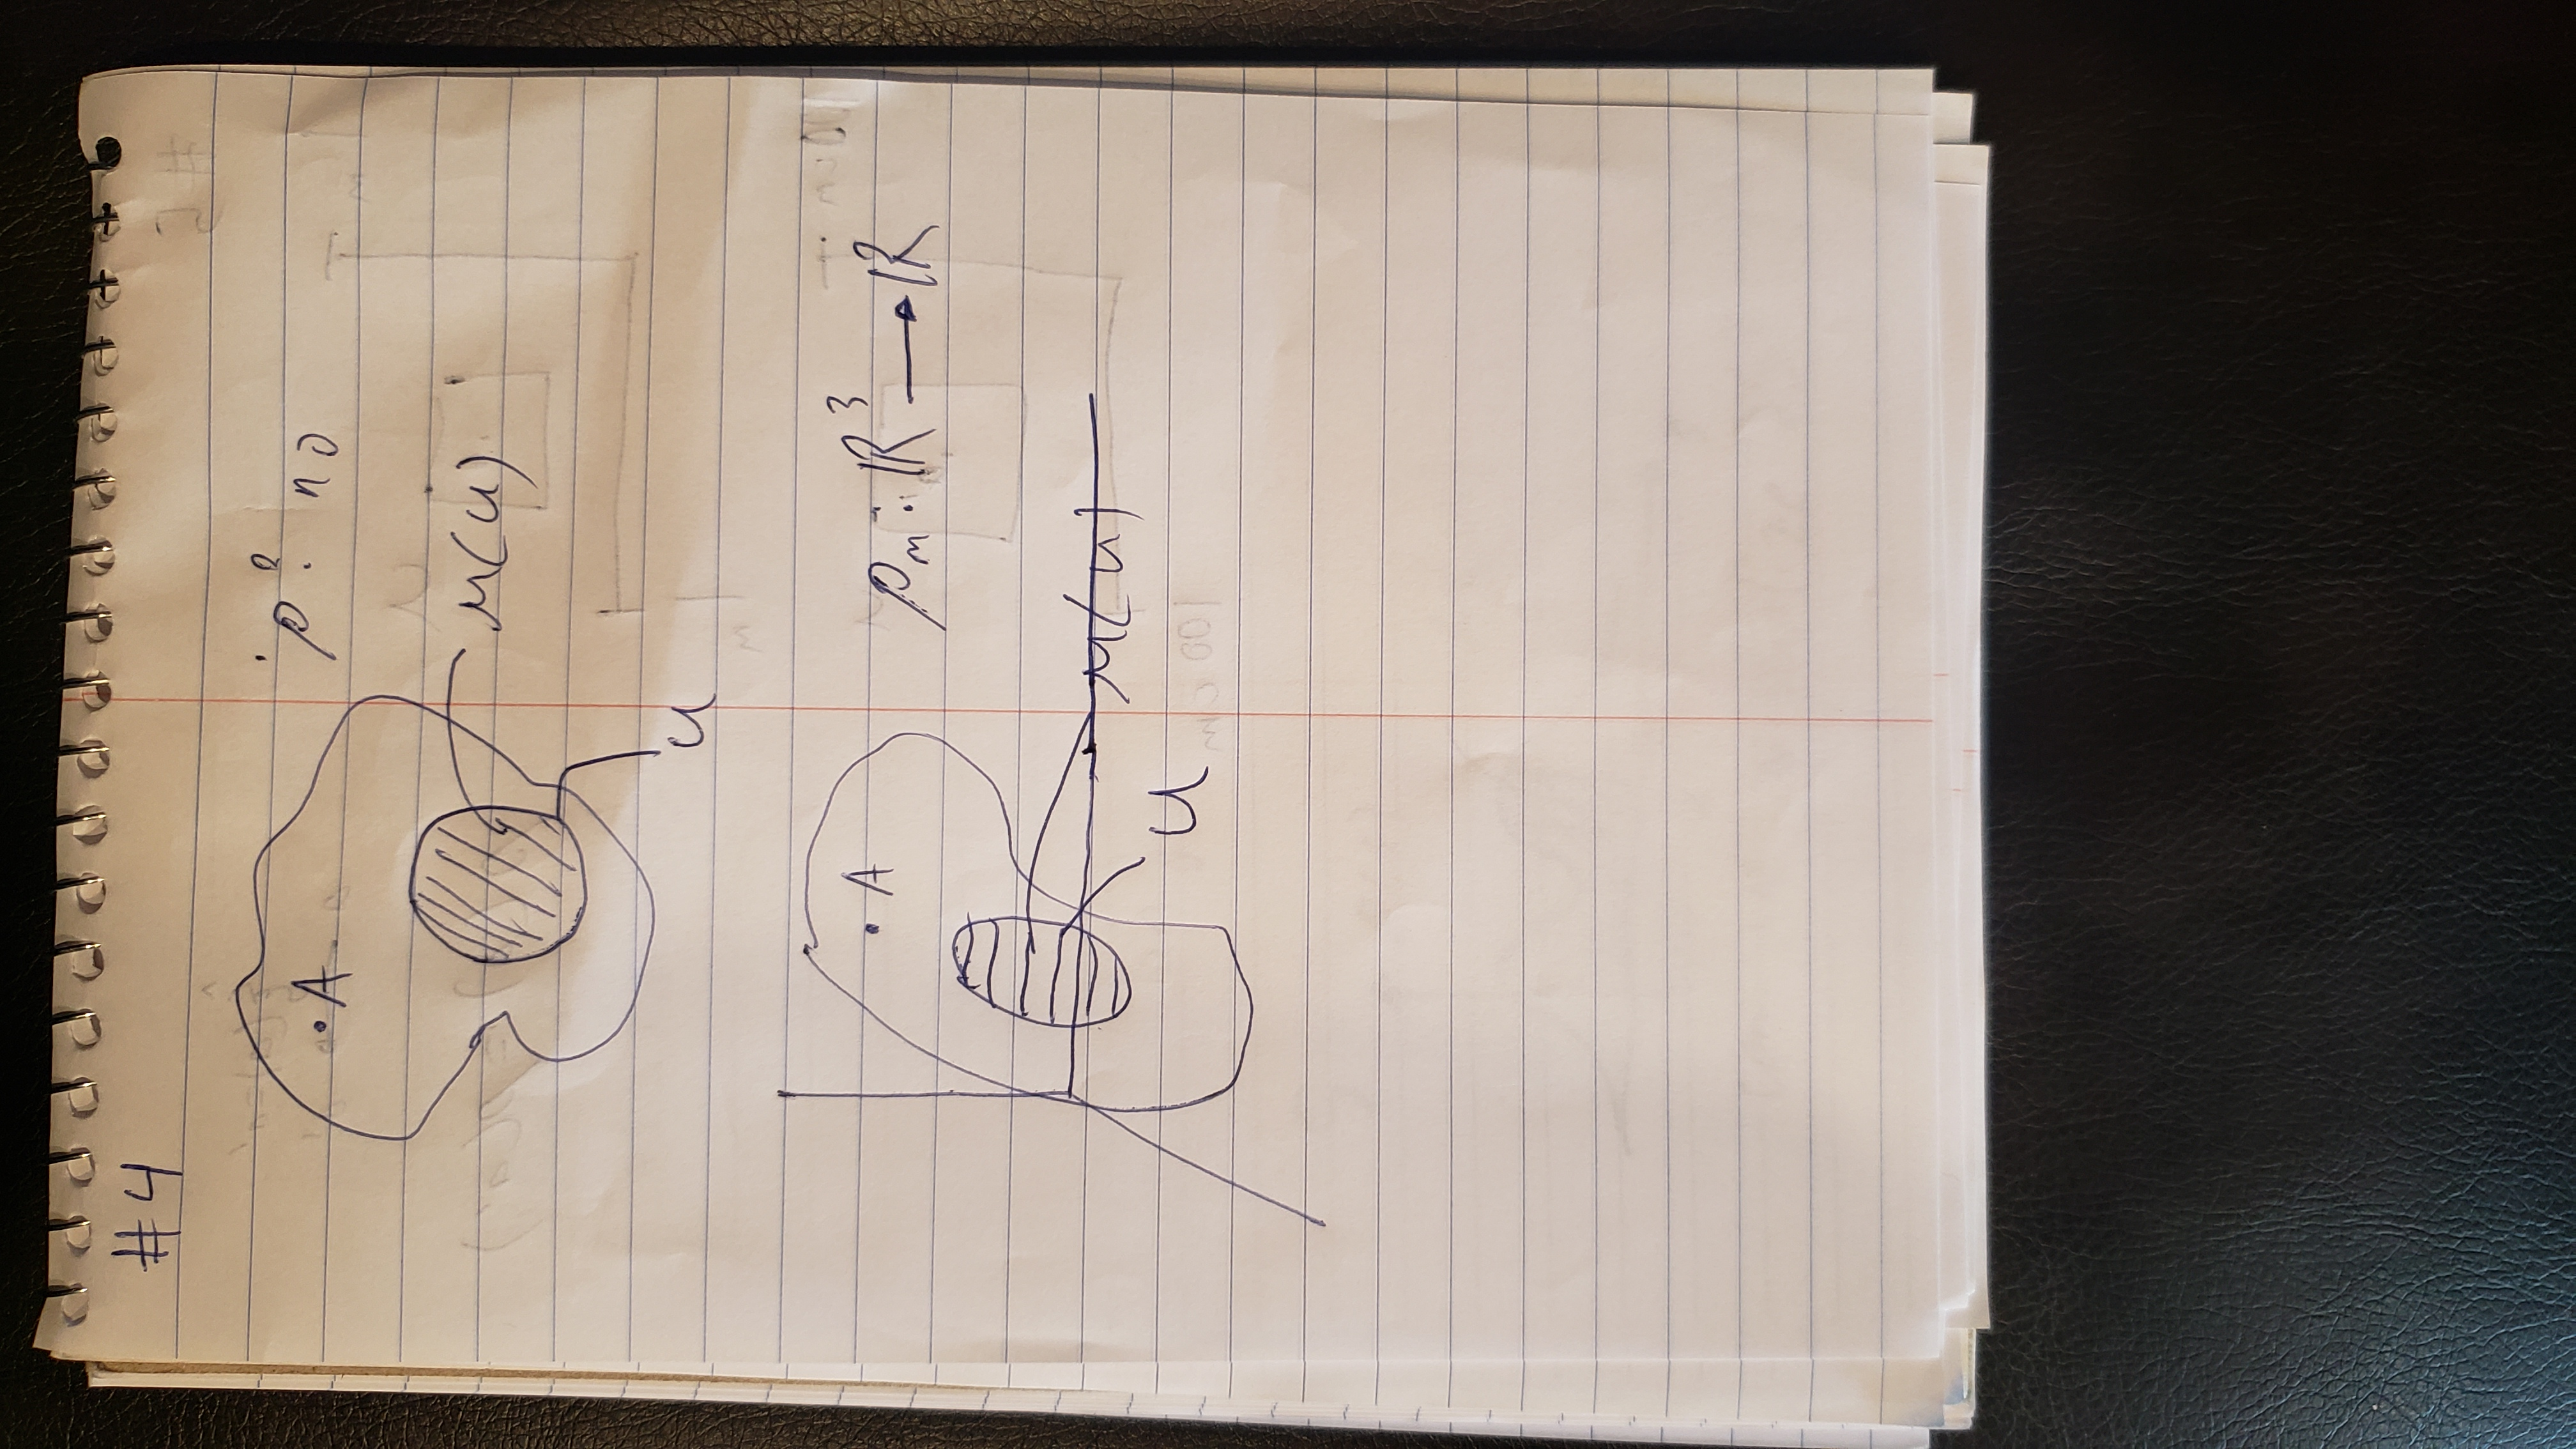
\includegraphics[width=\textwidth,angle=-90,scale=.45]{diagram4.jpg}}
\caption{One dimensional continuous example of our counting function $\mu(U)$.}
\end{figure}
	
\begin{defn}
	Let $\mathcal{C}$ be the state space of a system. The system is \textbf{infinitesimally reducible} to the infinitesimal parts (i.e. particles) identified by the state space $\mathcal{S}$ if there exists a measure $dS$ such that for every $c \in \mathcal{C}$ we can find a $\rho : \mathcal{S} \to \mathbb{R}$ such that for every $U \subseteq \mathcal{S}$ the integral $\mu(U) = \int_U \rho(s) dS$ corresponds to the fraction of the system whose parts occupy those states, which means $\mu(S) = 1$.
\end{defn}	
	
\subsection{Constraint on Coordinate Transformations}	
\iffalse
\begin{itemize}

\item We can now express density in terms of state variables. These state variables must be differentiable.

\item Prop - the state space must be a differentiable manifold

\item How should the change of state variable affect the density (units/value)?

\item On one side, it should be invariant. rho(s), like a temperate

\item On the other hand, units of the density are affected by the units of the state variables (mass example, include cart -> polar)

\item How do we solve this? Restrict state variable to "canonical", those that allow us to express the density in the correct units.

\item Jacobian must be unitary under canonical transformation

\item Prop - the state space must allow state variables that allow the expression of the density in the correct units (canoncial). Canonical transformations must have unitary and dimensionless Jacobian.
\end{itemize}
\fi

	%\emph{motivate necessity of labeling state space with numbers}
	%\emph{example and expand explanation. Discuss correct variables and set of quantities} 
	
	If we want to further describe the state of the system we need to identify our states in $\mathcal{S}$ with numbers so that all states are uniquely labeled. This system of labeling will give us our \textit{state variables}. For example imagine an ideal gas in a box. We know that we can describe the state of this gas by giving its pressure, temperature, or volume. By giving two of these quantities we have completely described the state of the gas as the third can be ascertained from knowledge of the other two through the ideal gas law. The state of the gas is uniquely determined by the values of two quantities. Thus we have a one to one map from the state space to the values of a set of numerical quantities. It is important to understand that there is a precise number of state variables that are correct to use in every case. If we were to also include the third quantity we would have introduced a redundant label. For each pressure-volume pair there is exactly one possible temperature so if we include temperature in our labeling we no longer have a one to one map between the state space and sets of values as some triplets do not correspond to possible states. For each state there is one well defined pressure-volume pair. 

\begin{defn}
	A state variable assigns one numerical quantity to each state. Formally, it is a map $\xi : \mathcal{S} \to \mathbb{R}$. A complete set of state variables fully identifies a state. Formally, it is an invertible  map $\xi^a : S \rightarrow \mathbb{R}^n $. This gives us a state space that is locally isomorphic to $\mathbb{R}^n$ thus our state space is an n-dimensional \textbf{manifold}.
\end{defn}

	%\emph{Write $\rho$ as a density. Clarify density vs distribution} 
		
	Expressing $\rho$ in terms of these state variables is the next natural step. Consider a cannon ball that is shot through the air. If the ball is spinning the position and momentum of each infinitesimal region of the ball will vary. Let the position and momentum in space be our state variables. The parts of the system will be distributed across these positions and momenta. Writing our distribution in terms of these variables will give us a density. This density is a map from our state variables to a numerical value that describes how much of the system occupies an infinitesimal region on this manifold. We know $\rho$ will be a map $\rho(\xi^a): \mathbb{R}^n \to \mathbb{R}$. Note that the density and the distribution are distinct functions; specifically the distribution is $\rho(s) : \mathcal{S} \to \mathbb{R}$ and the density is $\rho(\xi^a) : \mathbb{R}^n \to \mathbb{R}$. The density requires labeling the space with state variables to be defined while the distribution does not.\footnote{Note that we will use $\xi^a, \xi^b, \xi^c$ for state variables; $q^i, q^j, q^k$ for unit variables; $\xi^\alpha, \xi^\beta, \xi^\gamma$ for state variables that include time (i.e. four momentum). For distributions/densities we use $\rho$; where we need to distinguish between the two we will use $\rho(s)$ for the distribution and $\rho(\xi^a)$ for the density. States are indicated with $s$ and state variables with $\xi$. Note the duplicity of $\rho$, $s$, and $\xi$. We use $\xi^a(s)$ as $\mathcal{S} \to \mathbb{R}^n$; $s(\xi^a)$ as $\mathbb{R}^n \to \mathcal{S}$.
Thus we have the following identities: $\rho(s(\xi^a)) = \rho(\xi^a)$; $\rho(s) = \rho(s (\xi^a(s)))$.}

	%\emph{jacobian of density under coord change -> differentiability (value of density at origin)}

	Under a change of coordinates $\rho(\xi^a)$ must have a well defined transformation rule. For example say we have the density as a function of $x$ and $y$. Then if we change to polar coordinates we now have $\rho(r,\theta)$. We can then write $$\rho(x,y) = \rho(r,\theta)\begin{vmatrix}
\frac{\partial r}{\partial x} & \frac{\partial r}{\partial y} \\
\frac{\partial \theta}{\partial x} & \frac{\partial \theta}{\partial y}
\end{vmatrix}.$$ Evidently these partial derivatives need to be defined to have a well defined transformation of the value of $\rho$. In general our transformation rule is in the form $$\rho(\xi^a) = \rho(\hat{\xi}^b)\left|\frac{\partial\hat{\xi}^b}{\partial\xi^a}\right|.$$ In our example above we do have one point at which the transformation is not well defined: the origin. We do not have well defined partial derivatives at the origin as theta is not well defined at that point. Thus our density is not well defined at the origin in polar coordinates. We will require that any state variables labeling our state space be differentiable so that we can define changes of these variables without introducing values of the state variables where our density is not well defined. So our state space will be a manifold labeled by differentiable state variables.

\begin{prop}
	The state space of our classical particles $\mathcal{S}$ is an n-dimensional \textbf{differentiable manifold}.
\end{prop}

%\emph{give example of coordinate independent quantity to get reader to think about what that means; clarify independent/dependent vs invariant rho(x,y,z) vs T(A) T(x,y) = T(r,theta) vs rho with Jacobian}

	 As we saw above, the density $\rho(\xi^a)$ will be affected by the labeling of our state space, but we also know that our distribution, $\rho(s)$ is independent of our choice of state variables. This will give us another consideration when thinking about how $\rho$ transforms. We can see another example of a coordinate independent quantity with temperature. We can give the temperature at a point in space without a coordinate system; it is coordinate independent. Take a point $A$ in three-dimensional space. There is no need for a conception any other unit to define the temperature. Formally this means we can write $T(A): \mathcal{M} \to \mathbb{R}$; this is a direct map from space-time to a number, we do not need to label space-time using a coordinate system. This independence also means logically that changing our coordinate system does not change the numerical value of temperature at a point nor its units. We can write $T(A) = T(x,y) = T(r,\theta)$ meaning that as long as the point we are discussing remains the same, the value of $T$ is the same regardless of the choice of coordinates. So temperature is invariant under change of coordinates.\footnote{We say coordinate independent to mean can be defined without a specified coordinate system; to be coordinate invariant means there will be no change under a change of variables. Some coordinate dependent quantities are coordinate invariant, but coordinate independent quantities are always coordinate invariant.}
	 
	%\emph{$\rho$ must be invariant}
 
	We know that the amount of a system occupying a region of state space does not change with the variables we use to label that space. Our distribution $\rho(s)$ is coordinate independent thus it is unaffected  by the choice of state variables $\xi^a$. We want this invariance to translate to our density $\rho(\xi^a)$ meaning that under a change of state variables $\rho(\xi^a)$ will be invariant i.e. $\rho(s(\xi^a)) = \rho(s(\hat{\xi}^b))$.
	
	%\emph{explain solving these apparent contradictions}

	We have found two seemingly contradictory transformation rules for our density $\rho$. On one hand, $\rho$ must transform as a density i.e. its value will vary under a change of variables; on the other hand $\rho$ must be invariant in value and units under a change of variables. In order to reconcile this we must restrict which state variables we use to label our state space. We will throw out any choice of variables that do not produce a $\rho$ that obeys both of these restrictions.
	
%Diagram 4 here showing transform as density and invariance

\begin{prop}
	Because it is a density and is coordinate invariant, $\rho$ will transform as a scalar and a density under a change of state variables $\hat{\xi}^b = \hat{\xi}^b(\xi^a)$. The state variables that allow $\rho$ to be expressed in a way that satisfies these conditions are called \textbf{canonical variables}.
\end{prop}

	%\emph{the consequences from the above conclusions, simplify}

	We know we can write our counting function $\mu(U)$ in terms of our state variables as $\mu(U) = \int_{\xi(U)} \rho(\xi^a) \prod_a \xi^a$. If we change our state variables we know that that fraction of the system in a region $U \subset \mathcal{S}$ will not change meaning $\mu(U)$ must be invariant under such a change. Let $\hat{\xi}^b = \hat{\xi}^b(\xi^a)$ be our change of variables. This gives us $$\mu(U) = \int_{\xi(U)} \rho(\xi^a) \prod_a d\xi^a = \int_{\hat{\xi}(U)} \rho(\hat{\xi}^b) \prod_b d\hat{\xi}^b.$$ Let's think about this in more concrete terms. We know that to find the total mass in a region from a density we write the integral $$\int dm = \int \rho_m dV.$$ If we want to conserve the value of this integral under a change of variables we know that if $\rho_m$ changes the value of $dV$ must change accordingly. Proposition 4 however, tells us that the value of $\rho$ cannot change, thus we know the value of our 'volume' element $d\xi^a$ cannot change either.
	
	Using our transformation rule we can write $\int_{\hat{\xi}(U)} \rho(\hat{\xi}^b)d\hat{\xi}^b = \int_{\xi(U)} \rho(\hat{\xi}^b)\left|\frac{\partial\hat{\xi}^b}{\partial\xi^a}\right|d\xi^a = \int_{\xi(U)} \rho(\xi^a)d\xi^a$. We already know $\rho(\xi^a) = \rho(\hat{\xi}^b)$ by proposition [placeholder]; we can drop the integral to get $\rho(\xi^a) = \rho(\hat{\xi}^b)\left|\frac{\partial\hat{\xi}^b}{\partial\xi^a}\right|$ which implies that $\left|\frac{\partial\hat{\xi}^b}{\partial\xi^a}\right| = 1$. This means that the value of the volume element\footnote{this volume element describes volume on our manifold $\mathcal{S}$.} as expected doesn't change.
	
\begin{prop}
	The state space $\mathcal{S}$ must admit canonical state variables. A change of state variables must be differentiable and must have a unitary Jacobian i.e. $\left|\frac{\partial\hat{\xi}^b}{\partial\xi^a}\right| = 1$. Such a transformation is a \textbf{canonical transformation}.
\end{prop}

\begin{center}
\renewcommand{\arraystretch}{1.6}
 \begin{tabular}{p{0.1\textwidth} p{0.3\textwidth} p{0.5\textwidth}}
 \hline
 Symbol & Name & Description \\ [0.5ex] 
 \hline\hline
 $\mathcal{C}$ & State Space of Whole System & Contains all possible states of the whole system. Each state $c$ maps to a unique distribution $\rho(s)$\\ [2ex]
 \hline
 $\mathcal{S}$ & State Space of Classical Particles & Contains all possible states of the parts of the system. Particles are distributed according to $\rho(s)$. \\ [2ex]
 \hline
 $\mathcal{M}$ & Space-Time & Physical space. In our case three-dimensional without temporal axis. \\ [1ex] 
 \hline
 $\rho(s)$ & Distribution of States & $\mathcal{S} \to \mathbb{R}$ \\
 \hline
 $\rho(\xi^a)$ & Density of States & $\mathbb{R}^n \to \mathbb{R}$ \\
 \hline
 $\mu(U)$ & Counting function & $\mathbb{P}(\mathcal{S}) \to \begin{cases}
 \mathbb{Z} & \text{if \textrm{discrete}}\\
 \mathbb{R} & \textrm{if continuous} \end{cases}$ \\ [2.3ex]
 \hline
 $\xi^a$ & State variables & $\mathcal{S} \to \mathbb{R}^n$ \\
 \hline
 $\rho(\xi^a)$ & Density & $\mathbb{R}^n \to \mathbb{R}$ \\
 \hline
 $\hat{\xi}^b(\xi^a)$ & Change of Variables & $\mathbb{R}^n \to \mathbb{R}^n$ \\ [1ex] 
 \hline
\end{tabular}
\end{center}

\subsection{Unit Variables, Conjugate Pairs, and 2n Dimensional State Space}

\begin{itemize}
	\item Show that units are linked by a unit system. Not all unit for all quantities can be chosen independently. distance, time $\to$ velocity, acceleration; energy, entropy $\to$ temperature $\frac{\partial{S}}{\partial U} = \frac{1}{T}$. Some units are fundamental, some are derived.
	
	\item Therefore, there exists a subsets of state variables, that define the unit system. Call them q
	
	\item a change of units is a change only on the q.  The other variable will have a change of units that is derived from the fundamental unit. Independent units can be changed independently (they don't induce a change on the other fundamental units)
	
	\item Definition
	
	\item What are the relationships between units within state variable such that we can have canonical transformations. Start with set of variable with just one fundamental unit. Find that have only one state variable with derived units. That's the conjugate.
	
	\item General case of multiple independent units. Change one by one, find conjugates. State space is even dimensional.
	
	\item Proposition
	
\end{itemize}

	%\emph{Talk about unit system in general: some choices are free, some are dependent. Give example of dependent/independent unit variables (like velocity down). Dimensionless 1 math throws away units}

	We know that to define a density we need some kind of units that relate areas of the manifold to the fraction of the system found on the surface. We must remember that we are working with physical systems here. This means that the units of our state variables are important. Some of our state variables will define a unit and others will have their units derived from the units of other state variables. For example if distance in a direction is defined in terms of meters and time is defined in terms of seconds, velocity in that direction must be defined in meters per second and acceleration must be of units of meters per second squared. The units of velocity and acceleration are derived from the definition of the units of distance and time. Changing the definition of a fundamental unit will also change the definitions of all the units derived from it. 
	
	%\emph{example no. 2}
	
	Another example of this relationship between variables and their units is the set energy, entropy, and temperature. If we define the units of energy and entropy, we have no choice in the units of temperature because the relation $T dS = dU \to T = \frac{dU}{dS}$ ensures that the units of temperature are equivalent to the units of energy divided by the units of entropy. We could just as easily define the units of energy and temperature which would give us the units of entropy through the same relation.
	
	 We will define a \textit{unit system} using a subset of our state variables which we will call our \textit{unit variables}. These unit variables will define the fundamental units underlying all other state variables. Changing these unit variables will induce a change in all of the other state variables that rely on the definition of that unit. Take our distance, velocity, and acceleration example; if we change the units of distance from meters to light years, our definitions of velocity and acceleration must change as well, but our units of time remain unchanged. Conversely if we change our units of time, the units of velocity and acceleration will still change, but our unit of distance is unaffected. Unit variables are independent of one another. Ostensibly, the definitions of temperature and time have nothing to do with one another.  Generalizing this fact we see that if we change one unit variable we do not induce a change of variables in any other unit variables.

\begin{defn}
	We define a unit variable $q \in \xi^a$ as a state variable that is the definition of a unit. The subset of unit variables $q^i \subset \xi^a$ defines a unit system upon which the other state variables depend meaning that a transformation $\hat{q}^j = \hat{q}^j(q^i)$ induces a unique change of state variables $\hat{\xi}^b = \hat{\xi}^b(\xi^a)$. Unit variables are independent of one another.
\end{defn}

	%\emph{what actually happens under change of unit variables?}
	
	Now we must ask how a change of state variables should affect the units of our density $\rho(\xi^a)$. Let's consider a typical example of a density: mass distributed over three dimensional space $\mathcal{M}$. If I have a mass distribution, and I ask you how much mass is there in a region $U \subseteq \mathcal{M}$; your answer would likely be a number followed by a unit (alternatively you could give your answer as a fraction of the total mass of the system as we will see later). This response would be coordinate independent as the definition of $U$ does not require a coordinate system; your answer depends only on the defined region of interest and the units of mass; there is no dependence on the choice of coordinates used to describe the space. We can talk about points in this space without a defined coordinate system. Take a point $A \in \mathcal{M}$; this is the same point in all references, and we do not need to have a coordinate system defined to talk about point $A$. If I ask for the mass density at that point, however, I need to specify a quantity like $kg/m^3$. Formally, I have to specify the unit system of the space. In math terms this means that the density function is defined as $\rho_m : \mathbb{R}^3 \to \mathbb{R}$ not $\rho_m : \mathcal{M} \to \mathbb{R}$. We cannot define a map directly from $\mathcal{M}$ to $\mathbb{R}$ because without a well defined notion of distance, density makes no sense. If we were to change our unit system to $kg/cm^3$ the actual numerical value of the density at each point changes. The change of units labeling the space also mean that the units of the density change as well. Thus $\rho(\xi^a)$ will transform as a density, thus it must have these same properties. The unit system of the state space will determine the units used to describe density. 
	
	As we saw in section $2.1$ the Jacobian of a change of variables will give the transformation rule of the density; the transformation rule for the units of the density will similarly be given by the units of the Jacobian. But we also know that like our counting function $\mu(U)$, we want our density to be unaffected by changes in our state variables in both its value and units. Because we will only use canonical state variables, we have ensured that the Jacobian of a change of state variables will be \textit{unitary}. This means that not only will the value be equal to one, but also that it will be unit-less. This ensures that like our counting function, $\rho$ will have the same units after a change of variables. 
	
	 Continuing with our hypothetical change in variables we know that a change of unit variables will induce a unique change in the other state variables. Because this change is unique we need only specify a change in unit variables. 
	 
	 %So we will ourselves change only the unit variables; the other state variables must change in accordance with the new definitions of units such that the units of density do not change.
	
\begin{figure}[!ht]
\centerline{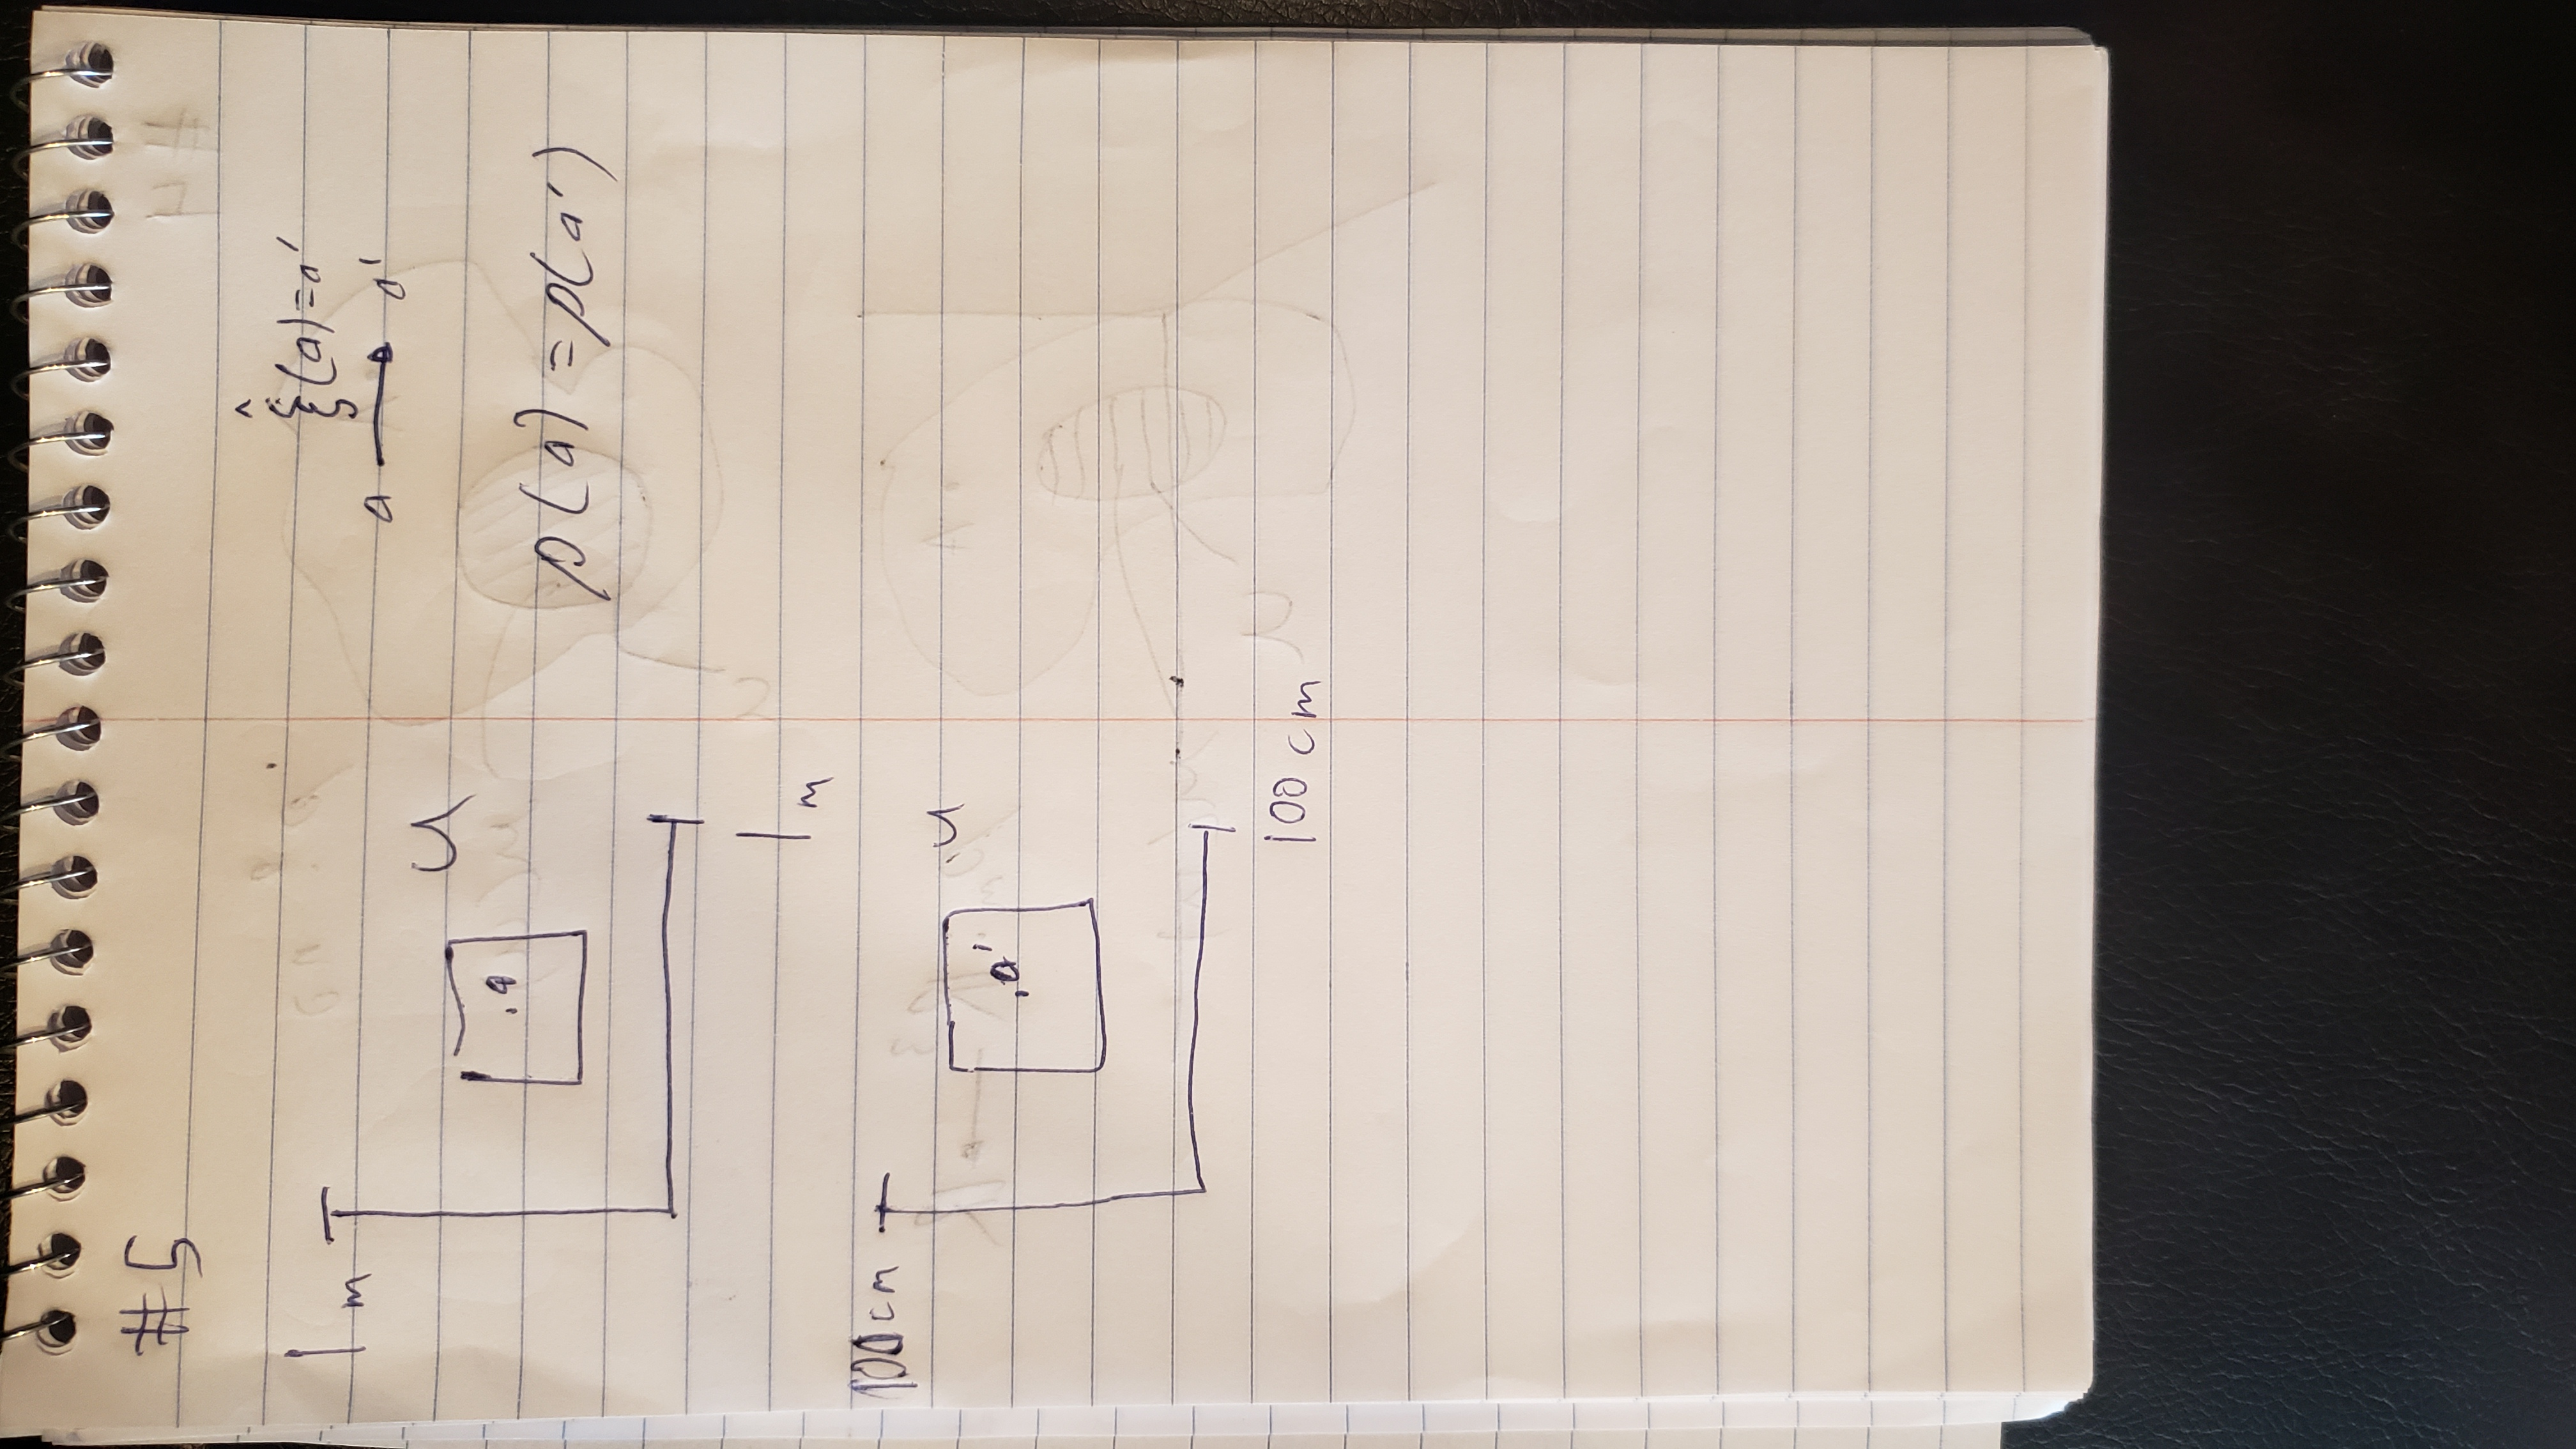
\includegraphics[width=\textwidth,angle=90,scale=.45]{diagram5.jpg}}
\caption{Visualization of the how the units with which we label our space affect the density. The important thing to note here is that while physically one meter and a hundred centimeters are the same, our mathematical system does not show this. This is where we as physicists must understand the differences between a physical system and a mathematical one.}
\end{figure}

	Now we will examine formally this change of units. Let's start with the simplest case: one unit variable suffices to describe our unit system. We then can write our set of state variables as $\xi^a = \{q,k^\mu\}$ where $k^\mu$ could represent any number of other state variables. Let's suppose we perform an arbitrary change of units. We then have $\hat{q} = \hat{q}(q)$. How must our set $\{k^\mu\}$ change while upholding our restriction to a unitary Jacobian? Our Jacobian block matrix will be of the form $$1 = \left|\frac{\partial\hat{\xi}^b}{\partial\xi^a}\right| = \begin{vmatrix}
\frac{\partial \hat{q}}{\partial q} & \frac{\partial \hat{q}}{\partial k^\mu} \\
\frac{\partial \hat{k}^\nu}{\partial q} & \frac{\partial \hat{k}^\nu}{\partial k^\mu}
\end{vmatrix}.$$

	If there are no $k^\mu$ variables then our constraint equation becomes $\left|\frac{\partial\hat{\xi}^b}{\partial\xi^a}\right| = \left|\frac{\partial \hat{q}}{\partial q}\right| = 1$. This does not allow us to make an arbitrary change in units meaning this case is invalid. We must have one or more $k^\mu$ variable(s).

	Because $\hat{q}$ has no dependence on $k^\mu$ we know that $\left|\frac{\partial \hat{q}}{\partial k^\mu}\right| = 0$. This means that our constraint becomes $\left|\frac{\partial \hat{q}}{\partial q}\right|\left|\frac{\partial \hat{k}^\nu}{\partial k^\mu}\right| = 1$. We know that $\hat{q}$ only depends on $q$ so we can write $(\left|\frac{d \hat{q}}{d q}\right|)^{-1} = \left|\frac{d q}{d \hat{q}}\right|$. We then get $\left|\frac{\partial \hat{k}^\nu}{\partial k^\mu}\right| = \left|\frac{d q}{d \hat{q}}\right|$. This provides only one constraint on our transformation. We know that we must have a unique transformation. So if we have two or more $k^\mu$ variables we cannot say that $q$ fully defines the unit system for all other state variables as a change in $q$ does not induce a unique change in the other state variables as it should. Thus we must have exactly one $k$ variable and our manifold will be two dimensional. This $k$ variable is called a \textit{conjugate variable}.
	
	What are the units of the conjugate variable $k$? Recall the earlier equality $\left|\frac{d\hat{q}}{dq}\right|\left|\frac{\partial \hat{k}}{\partial k}\right| = 1$. It is important that we know this equality gives us a unitless quantity. This means we can relate the units of $k$ to the units of $q$. We determined earlier that $k$ is a function only of $q$ and as such the units of $k$ written as $[k]$ must only be a function of the units of $q$. Rearranging the earlier equality gives us $$\left|\frac{d\hat{q}}{dq}\right| = \left|\frac{\partial k}{\partial \hat{k}}\right|$$. This means we will write the units of $k$ as $[k] = \frac{1}{[q]}$.
	
	%Recall the earlier equality $\left|\frac{d\hat{q}}{dq}\right|\left|\frac{\partial \hat{k}}{\partial k}\right| = 1$. Now suppose $q$ is defining a distance in meters and $\hat{q}$ defines distance in centimeters. This means the units of $\left|\frac{d\hat{q}}{dq}\right|$ would be $\frac{cm}{m}$. In order for the Jacobian to be unitary the units of $\left|\frac{\partial \hat{k}}{\partial k}\right|$ must then be $\frac{m}{cm}$. Now this allows us a choice of the units of $k$. The only restriction we have is that the units of $\frac{\hat{k}}{k}$ written as $\frac{[\hat{k}]}{[k]}$ must be $\frac{m}{cm}$. If the units of k were given as a density in kilograms per meter then the units of $\left|\frac{\partial \hat{k}}{\partial k}\right|$ would be $\frac{\frac{kg}{cm}}{\frac{kg}{m}}$ which would still result in a unitary Jacobian. By definition the units of $k$ only depend on the units of $q$. This means the units of $k$ are restricted to be precisely the inverse units of the corresponding $q$ i.e. $[k] = \frac{1}{[q]}$. Ostensibly we have a choice of the units of $k$ because we have a choice 

	How does this generalize to higher dimensions? Let's consider a state space whose unit system is described by $\{ q^i \}^n_{i=1}$ where each $q^i$ is an independent unit variable meaning a change in one of the unit variables will not affect in any way the other unit variables and that this change will be a function only of the original unit variable. Now we will perform individual changes of unit variables. We will write the first of these changes as $\hat{q}^1(q^1) = \hat{q}^1$. Writing this out explicitly (list of q hat changes) Because we are fixing all of the $\{ q^i \}^n_{i=2}$ variables this case is the same as the one unit variable system. This means that we will find precisely one conjugate $k_1$ variable that corresponds to $q^1$ whose units are the inverse of those of $q^1$. By continuing this process we arrive at the set of state variables given by $\{ q^i, k_i \}^n_{i=1}$ and a $2n$ dimension manifold.
\begin{prop}
	The state space of the particles is $2n$ dimensional. The state variables are organized in pairs $\{q^i, k_i\}$ where the set $\{q^n\}$ defines the unit system. These state variables have a well defined transformation rule with a unitary Jacobian.
\end{prop}

	%Now how do we ensure that our counting function $\mu(U)$ remains a pure number? We must constrain the units of our conjugate variables in order to do this. As we saw in figure [placeholder] a typical density changes as the variables used to label the space are changed. In our case however, we know that under a canonical change of variables our Jacobian is unitary. How can we understand this in terms of our change of units $\hat{q}^j = \hat{q}^j(q^i)$? We know we will have a corresponding change of conjugate variables $\hat{k}_j = \hat{k}_j(q^i,\hat{q}^j)$. We also know that the value of our volume element $d\xi^a = dq^i \land dk_i$ will not change in value or units. Thus we know that each $k_i$ must be of inverse units of its corresponding $q^i$. This means that any change in the unit variables $\{q^i\}$ will have a corresponding inverse change in conjugate variables $\{k_i\}$.\emph{change to differential justification}
	
	%\emph{needs work}	
	
	%Generalizing an equality we used earlier to higher dimensions gives $$\left|\frac{\partial \hat{k}_j}{\partial k_i}\right| = \left|\frac{d q^i}{d \hat{q}^j}\right|.$$ Evidently the change of units in $q^i$ induces an inverse change in the units of $k_i$. We know that the units of $k_i$ are only defined by the units of its corresponding $q^i$. We we know that the units of $k_i$ must be exactly the inverse units of $q^i$ i.e. $[k_i] = \frac{1}{[q^i]}$.
	
\begin{prop}
	The units of conjugate variables $\{k_i\}$ are the inverse of the units of the corresponding unit variables $\{q^i\}$. The volume element $d\xi^a = d\xi^{2n} = dq^n \land dk_n$ is invariant in value and units under a canonical change of variables.
\end{prop}

\subsection{Degrees of Freedom, Areas in State Space, and Poisson Brackets}
\begin{itemize}
	
	\item (assuming we established k is inverse units of q) We now fix the units to count states. In statistical mechanics, we use "hbar" to do that. An independent degree of freedom is a pair of variables as seen before. Therefore hbar dq dk measures states, therefore it is useful to define p = hbar k. P now depends on both the unit of q and the unit we used for the states.
	
	\item definition a degree of freedom is a pair of variable (q, p) such that dq dp = dS
	
	\item We want to characterize whether any pair of state variable can form an independent degree of freedom. We define an operator that takes two variables and returns the following. If the two variables cannot form a degree of freedom, for example, they are both defining an independent unit, then the operator returns 0. If they can define an independent degree of freedom, then they return the unit change of the area $df dg/dS$.
	
	\item Define $\{ f , g\}$ is an operator....
	
	\item Now, suppose we have canonical variable for all degrees of freedom $\{q^i, p_i\}$ such that $q^1$ and $p_1$ form the same degree of freedom identified by $f$ and $g$. Then there exists an invertible transformation that goes from one to the other. Therefore the poisson bracket is the Jacobian. If the d.o.f. is spread over multiple canonical variables, one finds that (sum over all d.o.f. of the canonical variables).
	
	\item Prop The Poisson bracket is sum of partials... (formula)
\end{itemize}

	We showed in section $2.1$ that the volume element expressed in canonical variables $\prod_a d \xi^{a} = d\xi^1 d\xi^2 \dots d \xi^{2n}$ is invariant under a canonical transformation. We want to relate this differential to our measure $dS$. How do the variables with which we label our state space relate to the number of possible states in that space? This requires a few considerations. What units will we use to count these states? The convention in statistical and quantum mechanics is to use $\hbar$ as the units of number of states; we will continue this convention. We define the units of our measure $dS$ to be $\hbar$. We write $p = \hbar k$ so that our new conjugate variable $p$ depends not only on the unit of $q$, but also on the units used to count states. Here we are exercising our freedom to choose the units of the conjugate variables. Recall the discussion earlier of the units of $k$. Instead of $\frac{kg}{m}$ we are giving $p$ the units of number of states over the unit of $q$. This choice allows us to relate the state variables labeling the space to the number of states contained in that space in a precise way. 
	
	In defining $p$ this way we arrive at the relation $dS = \prod \limits_{i = 1}^{n} dq^{i}dp_i$. From section $2.2$ we know that each conjugate variable is a function of one and only one unit variable. This means that each individual pair of $\{q^i,p_i\}$ variables will chart a 2D surface in phase space that can be described independently of the other state variables. We will call these pairings and the surfaces associated with them \textit{degrees of freedom}.

\begin{defn}
	A degree of freedom (d.o.f.) is a pair $\{q^i,p_i \}$ such that $dS^i = dq^i dp_i$. The measure $dS^i$ quantifies the number of possible configurations within an infinitesimal surface identified by that degree of freedom.
\end{defn}

	If we want to count the number of possible states over one d.o.f. we can integrate using the measure $dS$. The integral that gives the number of possible states in a region $U$ of our surface is $\int_{U} dq dp = \int_{U} dS$.

	How do we count states over multiple degrees of freedom? For example imagine we have a state space of four dimensions where $q^1,q^2$ are positions along the $x$ and $y$ axes and $p_1,p_2$ are momenta along those axes. The two pairings $\{q^1,p_1 \}$ and $\{q^2,p_2 \}$ are our degrees of freedom. We can count the total number of possible states by first counting the possible configurations of position and momentum in each dimension then multiplying these two counts together because the degrees of freedom are independent: the choice of a configuration in one has no effect on the choice of a configuration in the other. Thus the surfaces are orthogonal and the total number of possible states is given by the product of the possibilities in each degree of freedom.

\begin{defn}
	Two degrees of freedom are \textbf{independent} if the number of configurations identified by them is the product of the configurations identified by the individual degrees. That is, $dS = dS^1 dS^2$. Since the volume is the product of the areas, independent degrees of freedom are orthogonal.
\end{defn}

	How do we determine if a pair of variables forms a degree of freedom? Not all variables are compatible with each other. Consider our earlier example of 4D state space. We could not define the $x$-position and $y$-momentum as a degree of freedom because a change of units of the x position will not induce a change in the units of y momentum. To formalize this we will define an operator that tells us if two state variables are compatible.\footnote{This idea may feel familiar. That's because the operator we will define is classical equivalent of the quantum commutator.} This operator will take two state variables $f,g$ and return 0 if the variables are not compatible and do not form a d.o.f. or the unit change of the area $dfdg/dS$ if they are. This operator is called a \textit{Poisson bracket}.

\begin{defn}
	The Poisson bracket is defined as $\{f,g\} = \sum_i \frac{\partial f}{\partial q^i}\frac{\partial g}{\partial p_i} - \frac{\partial g}{\partial q^i}\frac{\partial f}{\partial p_i}$.
\end{defn}

	Let's suppose we have canonical variables for all our degrees of freedom $\{q^i,p_i\}$ such that $\{q^1,p_1\}$ form the same degree of freedom as our state variables $f$ and $g$. If $f$ and $g$ are canonical variables that form a d.o.f. then $\{f,g \} = dfdg/dS = 1$. If this operator returns a non-unitary value we know that $f$ and $g$ are not canonical variables. We know that because our degrees of freedom are independent and because we've limited ourselves to the use of differentiable state variables only, there will exist an invertible transformation between $f,g$ and $q,p$. If we recall that the Poisson bracket returns the unit change of area $dfdg/dS$, we see that the Jacobian of this transformation is precisely the Poisson bracket of $f$ and $g$.

\begin{prop}
	The Poisson bracket $\{f, g\}$ translates the densities of states into densities per unit area of $f, g$. It is the Jacobian of the transformation $dfdg \rightarrow dqdp$ i.e. $dfdg = \{f,g\}dqdp$.
\end{prop}
	
\section{Deterministic and Reversible Evolution}

\begin{itemize}
	\item Describe what deterministic and reversible mean. Bijection from past states to future states. Not enough.
	
	\item Example: damped harmonic oscillator. While the map is invertible, the density associated to the initial state is smaller than the final state.
	
	\item introduce the math (evolution, density over time)
	
	\item definition: define evolution, define density over time, define det/rev evolution as properties of evolution and density (i.e. density conservation)
	
	\item Show single degree of freedom. q and p variables. The evolution is both invertible (det/rev) and differential (because we need a Jaobian well defined). Because densities are conserved, divergence is zero. Displacement is the curl of a potential H. Get the equations.
	
	\item Generalizes by noting each infinitesimal surface maps to infinitesimal surfaces of the same area (same number of states). Independent d.o.f. remain independent (i.e. remain orthogonal).
	
	\item prop with equations
	
\end{itemize}


\begin{assump}[Deterministic and Reversible Evolution]
	The system undergoes deterministic and reversible evolution meaning given the state of the system at any time, its state at all past and future times is known.
\end{assump}

	We will now make an assumption about the time evolution of the system. The resulting mathematical structure will describe this evolution in terms of our state variables.

	For a system to undergo deterministic and reversible evolution there must be a bijection between all past and future states of the classical particles that make up the composite system. We must also have that the density of states, $\rho$ is conserved over time. Now this does not mean that our classical particles cannot change state. It means that if we have a certain number of classical particles in a initial state, all of those particles and no others will end up in the same final state.
	
	Why must we have the additional requirement of the conservation of the density when it seems the existence of the bijection would be sufficient for the evolution of our system to be deterministic and reversible? Here is an example of a system for which we can write a bijection, but for which the density of states is not conserved. We will see that the condition of the bijection is not strong enough to provide us with the desired mathematical structures.
	
	Imagine we have a one dimensional damped harmonic oscillator. We have a one to one map from past states to future states. But we also know that no matter the initial state, as the system evolves it will approach its rest state because it the oscillator is damped. Our state variables will be position and momentum. We know that in the real world all measurements have finite precision. This informational granularity tells us that at some point in the above example we will not be able to tell the difference between the state in which the oscillator  is barely moving and its rest state; a measurement will tell us that they are the same. Thinking of this in terms of our knowledge of the system we see that as time progress and our states collapse towards the rest state, we lose information about the system. This means in reality our system is not reversible because once it passes a certain point we cannot deduce the past state of the system from its current state; when the system is at rest we have no idea of its initial condition. Thus the addition of the requirement that density be conserved is necessary to ensure we can always deduce the past states of the system from its current state.
	
	Remember, this conservation does not mean that the classical particles cannot change states; it means only that if a certain number of particles begin in one state, that exact number of particles will end in the same state even if said final state is different from the original.
	
\begin{figure}[!ht]
\centerline{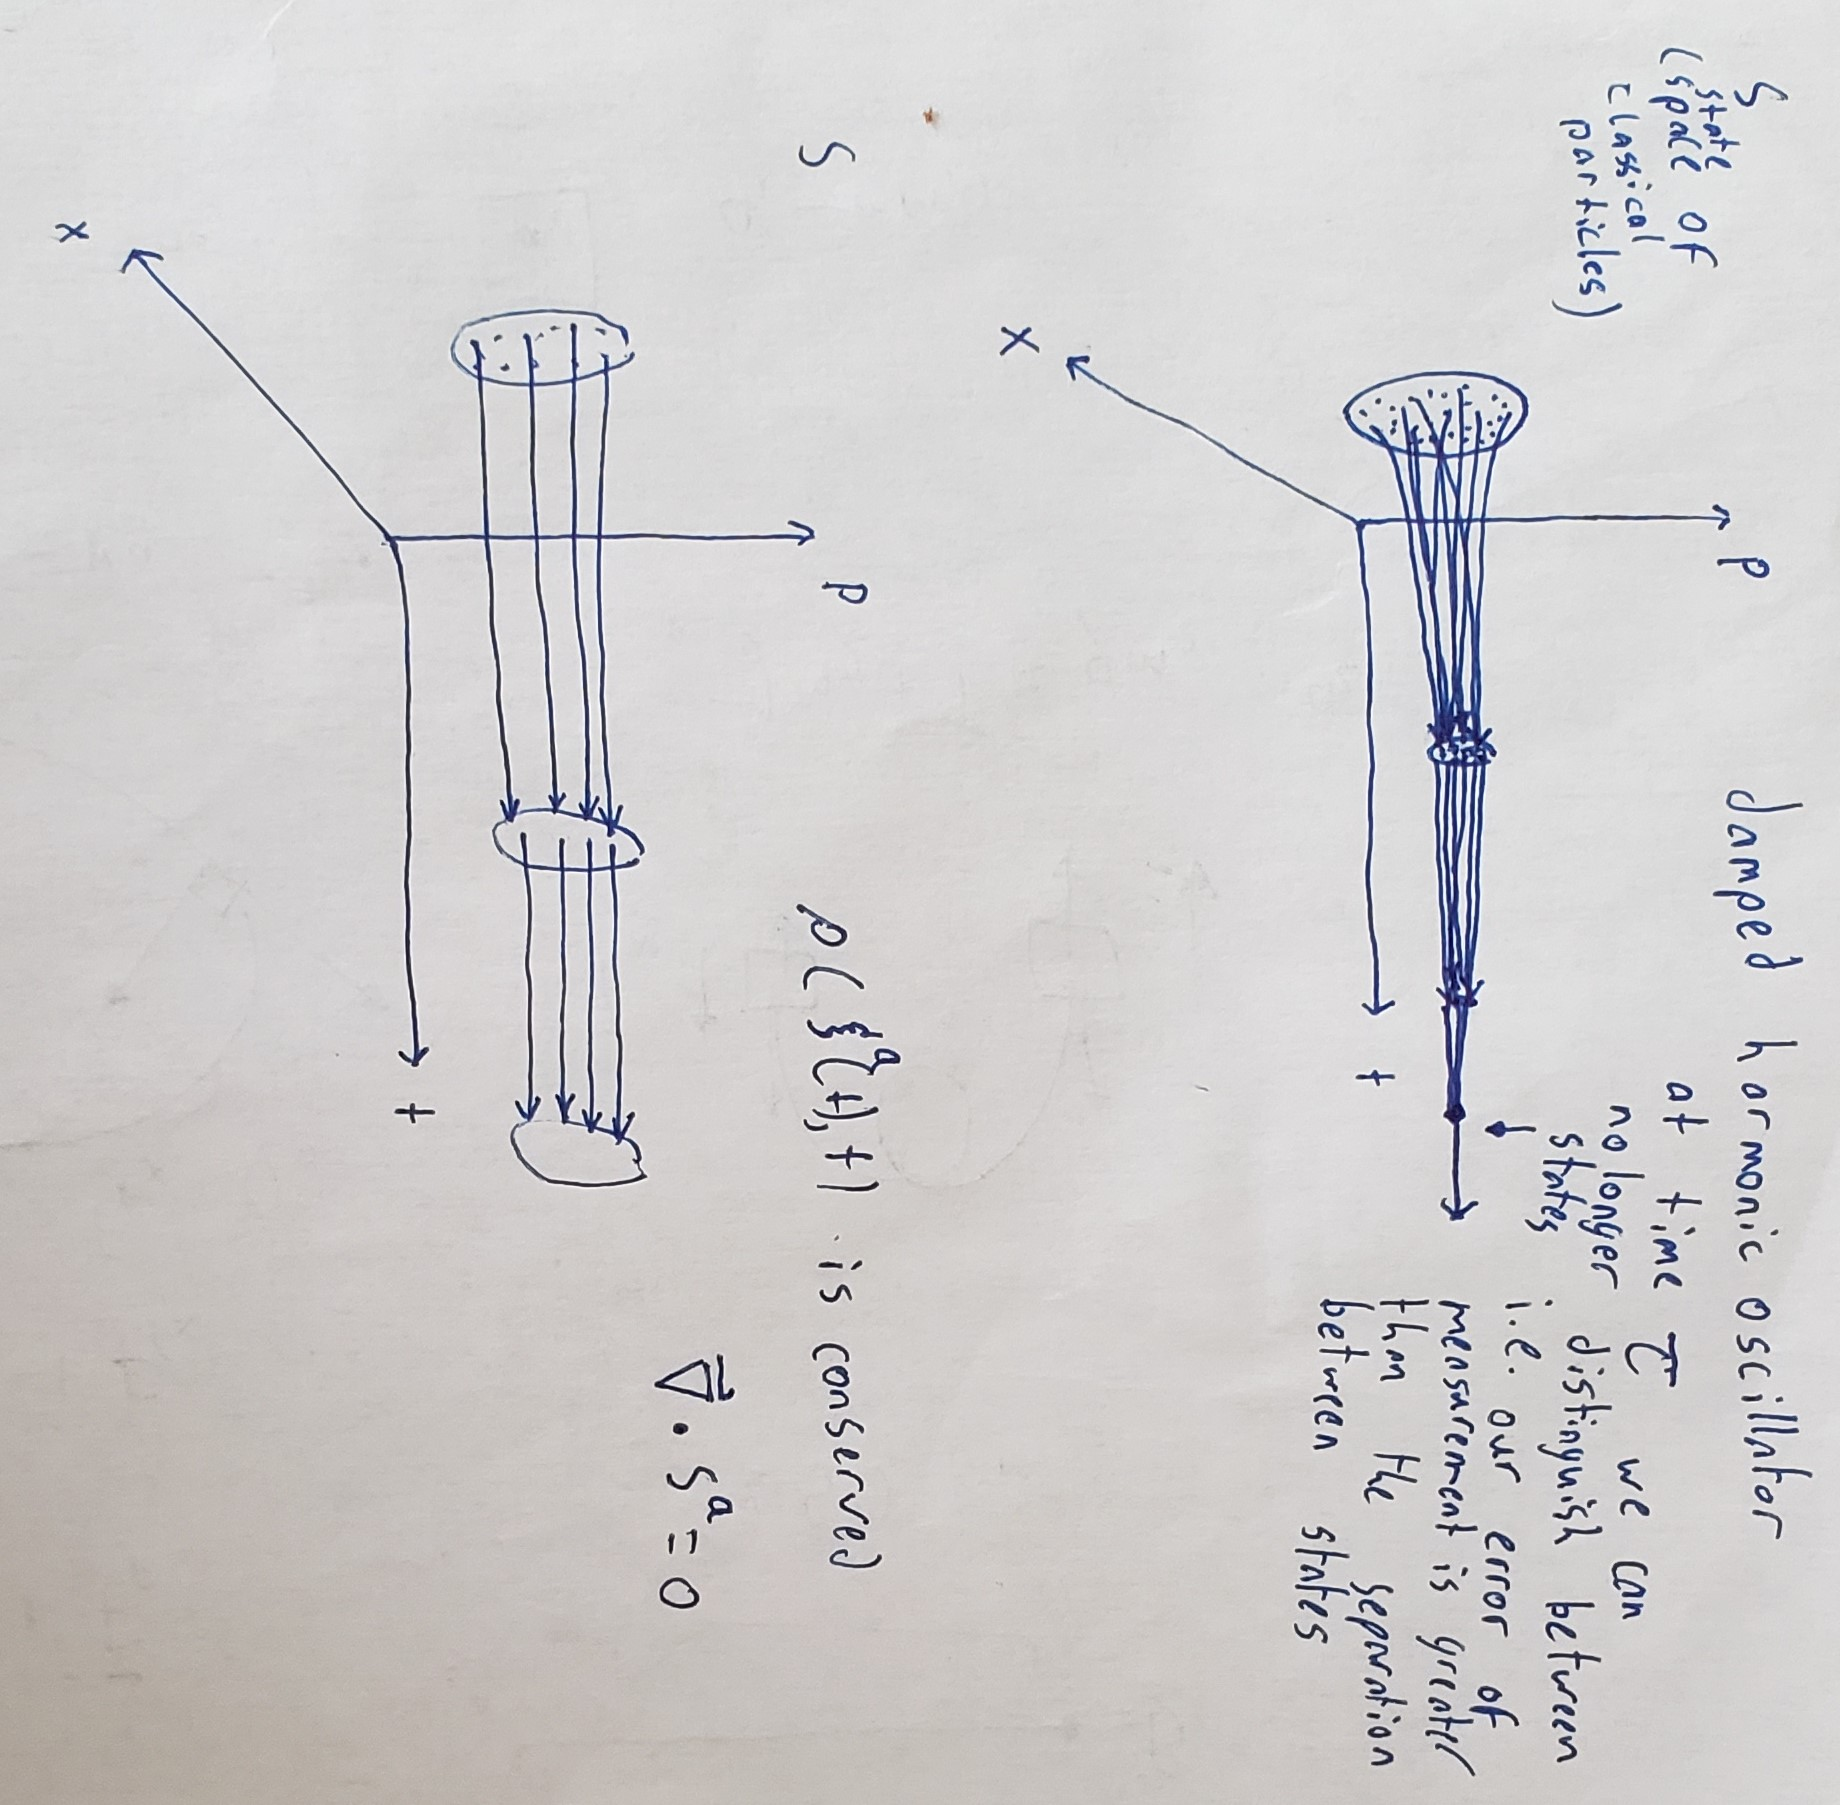
\includegraphics[width=\textwidth,angle=90,scale=.6]{streamfunctiondiagram.jpg}}
\caption{Bijection versus conservation of density illustrated by a retrodictable deterministic and reversible system that breaks down with informational granularity.}
\end{figure}

\begin{defn}
	A deterministic and reversible system is one for which all particles in a state are mapped to one and only one past or future state. That is, given a set of initial values $\xi^a_0$ at a time $t_0$, there is only one possible evolution $\xi^a(t)$ such that $\xi^a(t_0) = \xi^a_0$. Moreover, $\rho(\xi^a(t), t)$ is a constant.
\end{defn}

	We will continue to consider a system with a single degree of freedom and state variables $\{q,p \}$. If we transport our 2D state space in time $t$, we can map the evolution of each classical particle in $\mathbb{R}^3$. The evolution of the state of each particle can be written as $\xi^a(t)$ and the fraction of the system that is found in that state is $\rho(\xi^a(t), t)$. If we change infinitesimally in time we can write $\xi^a(t + dt) = \xi^a + \frac{d\xi^a}{dt}dt$. We know that $\xi^a(t)$ is differentiable because $\rho$ is always defined. We then will write a 2D vector field $S^a =\frac{d\xi^a}{dt} = \{\frac{dq}{dt},\frac{dp}{dt} \}$. In our damped oscillator example this vector field will have a nonzero divergence i.e. $\mathbf{\nabla} \cdot S^a =\mathbf{\nabla} \cdot \frac{d\xi^a}{dt} \neq 0$ because the states of the particles get closer together as the system tends towards its rest state as illustrated in the diagram above. With the requirement that $\rho(\xi,t)$ be conserved in time, we know that the divergence of this vector field is must be zero $$\mathbf{\nabla} \cdot S^a = \frac{\partial S^q}{\partial q} + \frac{\partial S^p}{\partial p} = 0$$. This means that we can write our vector field $S^a$ as the curl of a stream function by Helmholtz's theorem: $$S^a = -\mathbf{\nabla} \times \theta$$ where $\theta$ is our vector potential. Plugging this in we get: Finally we arrive at a familiar looking set of equations: $$d_t q = \partial _{p} H$$ $$d_t p = -\partial _q H.$$ These are the typical equations used in Hamiltonian mechanics for a system with two state variables.
	
	Let's generalize this to a system with n degrees of freedom. Recall that each infinitesimal surface in phase space is mapped to a surface of the same area; this means that the number of possible states remains the same and that independent degrees of freedom remain independent and thus their surfaces remain orthogonal. We can break down a higher dimensional system into its d.o.f.s in order to arrive at our final equation: $$d_tq^i = \partial_{p_i}H$$ $$d_tp_i = -\partial_{q^i}H.$$ This is the generalized form of Hamilton's equations. A system that evolves according to these equations is a Hamiltonian system.

\begin{prop}
	The deterministic and reversible evolution of an infinitesimally reducible system follows Hamilton's equations. So the evolution of the system can be written in the familiar way:
	$$d_tq^i = \partial_{p_i}H$$
	$$d_tp_i = -\partial_{q^i}H$$
\end{prop} 

\iffalse
\section{Kinematic Equivalence}

\begin{assump}[Kinematic Equivalence]
	(More physicsy) Trajectories in space-time suffice to recover trajectories in phase space. We know the precise trajectory in phase space given a trajectory in physical space-time; there is an invertible bijection between the two.(diagram showing bijection)
\end{assump}

\begin{itemize}
	\item Describe what kinematic equivalence is. Use the photon as a counter-example.
\end{itemize}

\subsection{Weak Equivalence}

\begin{itemize}
	\item By weak equivalence we mean that the trajectories of a single particle are enough to identify the state of the that particle. We are focusing only on a single particle.
	
	\item Introduce notation. We use q, p and x, v even though q and x both identify position. We do that because $\partial/\partial q$ is different from $\partial / \partial x$.
	
	\item velocity is a always function of position and momentum (because of determinism). But, it must be now invertible.
	
	\item This means the Hessian of the Hamiltonian is defined and non-zero everywhere. We can define a Lagrangian.
\end{itemize}

\begin{defn}
	We take $x^i = q^i$. We then define $v_i = d_tx^i$. Weak equivalence means $v_i(q^i, p_i)$ is invertible.
\end{defn}

(photon counter-example $v^i$ function only of $x^i$)

\begin{prop}
	A classical system that satisfies weak equivalence is a Lagrangian system. Formally, we can a define a Lagrangian $\mathcal{L}$ that is convex and has unique solutions.
\end{prop}

\subsection{Full Equivalence}

\begin{itemize}
	\item We now extend the requirement on the composite state. We look at the transformation rule of the density from q, p to x, v. We want the change of unit to be dependent on q only.
	
	\item This means the Hessian is dependent on q only and can be defined as $m g^{ij}$.
	
	\item Find that the Hamiltonian is the one of a massive particle under scalar and vector potential forces.
\end{itemize}

The units that are used to express the density on position and velocity must be dependent only on $q^i$ if they are to fully define the unit system.

\begin{defn}
	Full equivalence means that Kinematic Equivalence extends to the composite system. So we have $\rho(q^i,p_j) = \left|J\right|\rho(x^i,v^j) = \left|\frac{\partial v^i}{\partial p_j}\right|\rho(x^i,v^j)$. The Jacobian is only a function of $q^i$.
\end{defn}

\begin{prop}
	A system that satisfies full kinematic equivalence obeys the laws of massive particles under potential forces.
\end{prop}

\section{Advanced topics}

\subsection{Action Principle}

The action principle that many courses in mechanics take \emph{a priori} is simple a consequence of our assumptions. We can find a physical justification for our mathematical structures.

\subsection{Kinematic vs dynamics}

Differences between Newtonian/Lagrangian/Hamiltonian mechanics.

Show that they are inequivalent. Newtonian mechanics needs n functions to define the evolution while Lagrangian/Hamiltonian requires 1. All Lagrangians that have unique solution have a Hamiltonian. All Hamiltonians have unique solutions, but not necessarily a Lagrangian. (must follow discussion on the action principle) Mix with examples.

Kinematics and dynamics. Newtonian and Hamiltonian mechanics necessarily define both. Technically, Lagrangian mechanics is purely kinematic (equations are only in terms of position and velocity - you can't distinguish apparent forces from real forces). The only way to recover the dynamics is to assume the system is also Hamiltonian.

Kinematic aliasing (systems with different dynamics may have the same kinematics). Example of 3 different dynamics (friction, boosted, losing mass). This is confusing because, in some cases, you can treat non-conservative systems in Lagrangian mechanics as they look like conservative systems in a non-inertial frame (naturally, the Hamiltonian and the conjugate momentum will not correspond to what you expect).

How is kinematic aliasing resolved. Newtonian mechanics resolves kinematic aliasing by invoking inertial frames and by writing equations that are valid \emph{only} in inertial frames (you can distinguish apparent forces from real forces in an inertial frame).  In Lagrangian/Hamiltonian mechanics, the equations are invariant under coordinate transformation: we can't do that anymore. You fix the system to be conservative. If you had a system of equations that were invariant under all coordinate transformation for all frames, you would not be able to tell which forces are apparent and which forces are real.

\subsection{Entropy in classical mechanics}

Entropy is invariant under coordinate transformation - the same for all observers (invariance under time is less important).

Classical uncertainty principle: fixing the entropy of the distribution gives us an inequality that is saturated by Gaussian distributions. (discuss parallel with quantum mechanics - classical mechanics allow for minus infinite entropy)

Time evolution of entropy. It is conserved only under Hamiltonian evolution. If the evolution is not Hamiltonian, the entropy does the opposite of what one expected. (dissipative systems, like damped harmonic oscillator, concentrate the distributions around the attractor, and therefore) The problem is that the same statement at different time provides different amount of information/granularity of the description.
\fi

\section{Conclusion}
	
\begin{itemize}

	\item start with assumptions discuss results

\end{itemize}


\bibliographystyle{acm}
\bibliography{Bibliography}















\end{document}
